\documentclass[11pt,a4paper]{article}
\usepackage[utf8]{inputenc}
\usepackage[T1]{fontenc}
\usepackage{lmodern}
\usepackage[margin=1in]{geometry}
\usepackage{amsmath,amssymb,amsthm}
\usepackage{booktabs}
\usepackage{graphicx}
\usepackage{microtype}
\usepackage[numbers,sort&compress]{natbib}
\usepackage{xcolor}
\usepackage[colorlinks=true,linkcolor=blue!50!black,citecolor=blue!50!black,urlcolor=blue!50!black]{hyperref}
\usepackage{enumitem}
\usepackage{array}
\usepackage{caption}
\captionsetup{font=small,labelfont=bf}

\IfFileExists{numbers.tex}{% generated by experiments/make_numbers.py -- do not edit
\newcommand{\MetaSeed}{20260930}
\newcommand{\MetaPython}{3.11.15}
\newcommand{\MetaNumpy}{2.4.6}
\newcommand{\MetaSklearn}{1.9.1}
\newcommand{\MetaScipy}{1.17.1}
\newcommand{\MetaSecondsMain}{231}
\newcommand{\MetaSecondsExact}{28}
\newcommand{\MetaSecondsTotal}{259}
\newcommand{\NDatasets}{6}
\newcommand{\NMainFolds}{10}
\newcommand{\NMainRepeats}{2}
\newcommand{\NRobFolds}{5}
\newcommand{\NoiseRate}{20}
\newcommand{\NoiseProb}{0.2}
\newcommand{\SubFrac}{25}
\newcommand{\InnerFolds}{3}
\newcommand{\KnnValCap}{40}
\newcommand{\KnnKs}{5, 10, 20, 50, 100}
\newcommand{\KnnC}{1}
\newcommand{\VbKbw}{10}
\newcommand{\VbBetas}{0, 0.5, 1}
\newcommand{\GammaMults}{0.1, 0.3, 1, 3, 10, 30, 100}
\newcommand{\GammaMultMax}{100}
\newcommand{\CRbf}{0.1, 1, 10, 100, 1000}
\newcommand{\CRbfMax}{1000}
\newcommand{\CLin}{0.001, 0.01, 0.1, 1, 10}
\newcommand{\CellMs}{1, 2, 4, 8, 16, 32}
\newcommand{\CellMMax}{32}
\newcommand{\CellCs}{0.1, 1, 10}
\newcommand{\LlsvmMs}{1, 2, 4, 8, 16, 32}
\newcommand{\LlsvmCs}{0.01, 0.1, 1, 10}
\newcommand{\KnnKMin}{5}
\newcommand{\NWine}{178}
\newcommand{\DWine}{13}
\newcommand{\NTrainMainWine}{142}
\newcommand{\NTrainSubWine}{40}
\newcommand{\NBc}{300}
\newcommand{\DBc}{30}
\newcommand{\NTrainMainBc}{240}
\newcommand{\NTrainSubBc}{60}
\newcommand{\NDig}{400}
\newcommand{\DDig}{64}
\newcommand{\NTrainMainDig}{320}
\newcommand{\NTrainSubDig}{80}
\newcommand{\NGauss}{400}
\newcommand{\DGauss}{10}
\newcommand{\NTrainMainGauss}{320}
\newcommand{\NTrainSubGauss}{80}
\newcommand{\NMoons}{400}
\newcommand{\DMoons}{2}
\newcommand{\NTrainMainMoons}{320}
\newcommand{\NTrainSubMoons}{80}
\newcommand{\NCheck}{400}
\newcommand{\DCheck}{2}
\newcommand{\NTrainMainCheck}{320}
\newcommand{\NTrainSubCheck}{80}
\newcommand{\AccMainWineLin}{99.2}
\newcommand{\AccMainWineRbf}{99.7}
\newcommand{\AccMainWineBest}{99.7}
\newcommand{\AccMainWineKnn}{99.4}
\newcommand{\AccMainWineCell}{98.3}
\newcommand{\AccMainWineVb}{99.7}
\newcommand{\AccMainWineLlsvm}{99.2}
\newcommand{\DiffMainWineKnn}{-0.28}
\newcommand{\DiffLoMainWineKnn}{-1.11}
\newcommand{\DiffHiMainWineKnn}{+0.56}
\newcommand{\LocalFracMainWineKnn}{60}
\newcommand{\DiffMainWineCell}{-1.42}
\newcommand{\DiffLoMainWineCell}{-2.83}
\newcommand{\DiffHiMainWineCell}{-0.01}
\newcommand{\LocalFracMainWineCell}{70}
\newcommand{\DiffMainWineVb}{+0.00}
\newcommand{\DiffLoMainWineVb}{+0.00}
\newcommand{\DiffHiMainWineVb}{+0.00}
\newcommand{\LocalFracMainWineVb}{0}
\newcommand{\DiffMainWineLlsvm}{-0.57}
\newcommand{\DiffLoMainWineLlsvm}{-1.67}
\newcommand{\DiffHiMainWineLlsvm}{+0.54}
\newcommand{\LocalFracMainWineLlsvm}{50}
\newcommand{\PickRbfMainWine}{100}
\newcommand{\AccMainBcLin}{96.0}
\newcommand{\AccMainBcRbf}{96.0}
\newcommand{\AccMainBcBest}{96.5}
\newcommand{\AccMainBcKnn}{95.2}
\newcommand{\AccMainBcCell}{96.2}
\newcommand{\AccMainBcVb}{96.0}
\newcommand{\AccMainBcLlsvm}{96.2}
\newcommand{\DiffMainBcKnn}{-1.33}
\newcommand{\DiffLoMainBcKnn}{-3.34}
\newcommand{\DiffHiMainBcKnn}{+0.67}
\newcommand{\LocalFracMainBcKnn}{40}
\newcommand{\DiffMainBcCell}{-0.33}
\newcommand{\DiffLoMainBcCell}{-1.33}
\newcommand{\DiffHiMainBcCell}{+0.50}
\newcommand{\LocalFracMainBcCell}{30}
\newcommand{\DiffMainBcVb}{-0.50}
\newcommand{\DiffLoMainBcVb}{-1.33}
\newcommand{\DiffHiMainBcVb}{+0.00}
\newcommand{\LocalFracMainBcVb}{30}
\newcommand{\DiffMainBcLlsvm}{-0.33}
\newcommand{\DiffLoMainBcLlsvm}{-1.50}
\newcommand{\DiffHiMainBcLlsvm}{+0.67}
\newcommand{\LocalFracMainBcLlsvm}{70}
\newcommand{\PickRbfMainBc}{70}
\newcommand{\AccMainDigLin}{85.2}
\newcommand{\AccMainDigRbf}{97.5}
\newcommand{\AccMainDigBest}{97.5}
\newcommand{\AccMainDigKnn}{98.2}
\newcommand{\AccMainDigCell}{95.5}
\newcommand{\AccMainDigVb}{97.6}
\newcommand{\AccMainDigLlsvm}{96.4}
\newcommand{\DiffMainDigKnn}{+0.75}
\newcommand{\DiffLoMainDigKnn}{-0.50}
\newcommand{\DiffHiMainDigKnn}{+2.00}
\newcommand{\LocalFracMainDigKnn}{100}
\newcommand{\DiffMainDigCell}{-2.00}
\newcommand{\DiffLoMainDigCell}{-3.50}
\newcommand{\DiffHiMainDigCell}{-0.37}
\newcommand{\LocalFracMainDigCell}{100}
\newcommand{\DiffMainDigVb}{+0.13}
\newcommand{\DiffLoMainDigVb}{-0.37}
\newcommand{\DiffHiMainDigVb}{+0.75}
\newcommand{\LocalFracMainDigVb}{50}
\newcommand{\DiffMainDigLlsvm}{-1.13}
\newcommand{\DiffLoMainDigLlsvm}{-2.25}
\newcommand{\DiffHiMainDigLlsvm}{-0.13}
\newcommand{\LocalFracMainDigLlsvm}{100}
\newcommand{\PickRbfMainDig}{100}
\newcommand{\AccMainGaussLin}{93.9}
\newcommand{\AccMainGaussRbf}{93.5}
\newcommand{\AccMainGaussBest}{93.3}
\newcommand{\AccMainGaussKnn}{90.6}
\newcommand{\AccMainGaussCell}{93.0}
\newcommand{\AccMainGaussVb}{93.6}
\newcommand{\AccMainGaussLlsvm}{93.1}
\newcommand{\DiffMainGaussKnn}{-2.62}
\newcommand{\DiffLoMainGaussKnn}{-3.88}
\newcommand{\DiffHiMainGaussKnn}{-1.62}
\newcommand{\LocalFracMainGaussKnn}{50}
\newcommand{\DiffMainGaussCell}{-0.25}
\newcommand{\DiffLoMainGaussCell}{-1.12}
\newcommand{\DiffHiMainGaussCell}{+0.50}
\newcommand{\LocalFracMainGaussCell}{30}
\newcommand{\DiffMainGaussVb}{+0.37}
\newcommand{\DiffLoMainGaussVb}{+0.12}
\newcommand{\DiffHiMainGaussVb}{+0.75}
\newcommand{\LocalFracMainGaussVb}{60}
\newcommand{\DiffMainGaussLlsvm}{-0.12}
\newcommand{\DiffLoMainGaussLlsvm}{-0.87}
\newcommand{\DiffHiMainGaussLlsvm}{+0.63}
\newcommand{\LocalFracMainGaussLlsvm}{90}
\newcommand{\PickRbfMainGauss}{80}
\newcommand{\AccMainMoonsLin}{84.5}
\newcommand{\AccMainMoonsRbf}{97.0}
\newcommand{\AccMainMoonsBest}{97.0}
\newcommand{\AccMainMoonsKnn}{96.6}
\newcommand{\AccMainMoonsCell}{93.2}
\newcommand{\AccMainMoonsVb}{97.1}
\newcommand{\AccMainMoonsLlsvm}{89.6}
\newcommand{\DiffMainMoonsKnn}{-0.37}
\newcommand{\DiffLoMainMoonsKnn}{-1.63}
\newcommand{\DiffHiMainMoonsKnn}{+1.00}
\newcommand{\LocalFracMainMoonsKnn}{100}
\newcommand{\DiffMainMoonsCell}{-3.75}
\newcommand{\DiffLoMainMoonsCell}{-5.88}
\newcommand{\DiffHiMainMoonsCell}{-1.25}
\newcommand{\LocalFracMainMoonsCell}{100}
\newcommand{\DiffMainMoonsVb}{+0.12}
\newcommand{\DiffLoMainMoonsVb}{-1.25}
\newcommand{\DiffHiMainMoonsVb}{+1.37}
\newcommand{\LocalFracMainMoonsVb}{100}
\newcommand{\DiffMainMoonsLlsvm}{-7.38}
\newcommand{\DiffLoMainMoonsLlsvm}{-9.13}
\newcommand{\DiffHiMainMoonsLlsvm}{-5.75}
\newcommand{\LocalFracMainMoonsLlsvm}{100}
\newcommand{\PickRbfMainMoons}{100}
\newcommand{\AccMainCheckLin}{50.8}
\newcommand{\AccMainCheckRbf}{89.4}
\newcommand{\AccMainCheckBest}{89.4}
\newcommand{\AccMainCheckKnn}{85.9}
\newcommand{\AccMainCheckCell}{81.7}
\newcommand{\AccMainCheckVb}{89.9}
\newcommand{\AccMainCheckLlsvm}{84.5}
\newcommand{\DiffMainCheckKnn}{-3.50}
\newcommand{\DiffLoMainCheckKnn}{-6.38}
\newcommand{\DiffHiMainCheckKnn}{-0.50}
\newcommand{\LocalFracMainCheckKnn}{100}
\newcommand{\DiffMainCheckCell}{-7.63}
\newcommand{\DiffLoMainCheckCell}{-11.38}
\newcommand{\DiffHiMainCheckCell}{-3.25}
\newcommand{\LocalFracMainCheckCell}{100}
\newcommand{\DiffMainCheckVb}{+0.50}
\newcommand{\DiffLoMainCheckVb}{-0.50}
\newcommand{\DiffHiMainCheckVb}{+2.12}
\newcommand{\LocalFracMainCheckVb}{50}
\newcommand{\DiffMainCheckLlsvm}{-4.88}
\newcommand{\DiffLoMainCheckLlsvm}{-7.63}
\newcommand{\DiffHiMainCheckLlsvm}{-1.87}
\newcommand{\LocalFracMainCheckLlsvm}{100}
\newcommand{\PickRbfMainCheck}{100}
\newcommand{\AccNoiseWineLin}{97.8}
\newcommand{\AccNoiseWineRbf}{97.7}
\newcommand{\AccNoiseWineBest}{97.7}
\newcommand{\AccNoiseWineKnn}{94.9}
\newcommand{\AccNoiseWineCell}{96.6}
\newcommand{\AccNoiseWineVb}{97.2}
\newcommand{\AccNoiseWineLlsvm}{97.7}
\newcommand{\DiffNoiseWineKnn}{-2.83}
\newcommand{\DiffLoNoiseWineKnn}{-5.70}
\newcommand{\DiffHiNoiseWineKnn}{-0.56}
\newcommand{\LocalFracNoiseWineKnn}{20}
\newcommand{\DiffNoiseWineCell}{-1.13}
\newcommand{\DiffLoNoiseWineCell}{-3.95}
\newcommand{\DiffHiNoiseWineCell}{+1.16}
\newcommand{\LocalFracNoiseWineCell}{80}
\newcommand{\DiffNoiseWineVb}{-0.57}
\newcommand{\DiffLoNoiseWineVb}{-1.71}
\newcommand{\DiffHiNoiseWineVb}{+0.00}
\newcommand{\LocalFracNoiseWineVb}{40}
\newcommand{\DiffNoiseWineLlsvm}{+0.00}
\newcommand{\DiffLoNoiseWineLlsvm}{+0.00}
\newcommand{\DiffHiNoiseWineLlsvm}{+0.00}
\newcommand{\LocalFracNoiseWineLlsvm}{60}
\newcommand{\PickRbfNoiseWine}{100}
\newcommand{\AccNoiseBcLin}{92.3}
\newcommand{\AccNoiseBcRbf}{90.3}
\newcommand{\AccNoiseBcBest}{91.7}
\newcommand{\AccNoiseBcKnn}{87.0}
\newcommand{\AccNoiseBcCell}{91.3}
\newcommand{\AccNoiseBcVb}{89.7}
\newcommand{\AccNoiseBcLlsvm}{92.7}
\newcommand{\DiffNoiseBcKnn}{-4.67}
\newcommand{\DiffLoNoiseBcKnn}{-8.00}
\newcommand{\DiffHiNoiseBcKnn}{-0.33}
\newcommand{\LocalFracNoiseBcKnn}{60}
\newcommand{\DiffNoiseBcCell}{-0.33}
\newcommand{\DiffLoNoiseBcCell}{-1.00}
\newcommand{\DiffHiNoiseBcCell}{+0.00}
\newcommand{\LocalFracNoiseBcCell}{60}
\newcommand{\DiffNoiseBcVb}{-2.00}
\newcommand{\DiffLoNoiseBcVb}{-3.00}
\newcommand{\DiffHiNoiseBcVb}{-1.00}
\newcommand{\LocalFracNoiseBcVb}{20}
\newcommand{\DiffNoiseBcLlsvm}{+1.00}
\newcommand{\DiffLoNoiseBcLlsvm}{+0.00}
\newcommand{\DiffHiNoiseBcLlsvm}{+3.00}
\newcommand{\LocalFracNoiseBcLlsvm}{40}
\newcommand{\PickRbfNoiseBc}{40}
\newcommand{\AccNoiseDigLin}{81.8}
\newcommand{\AccNoiseDigRbf}{84.5}
\newcommand{\AccNoiseDigBest}{83.5}
\newcommand{\AccNoiseDigKnn}{80.7}
\newcommand{\AccNoiseDigCell}{83.0}
\newcommand{\AccNoiseDigVb}{85.0}
\newcommand{\AccNoiseDigLlsvm}{85.5}
\newcommand{\DiffNoiseDigKnn}{-2.75}
\newcommand{\DiffLoNoiseDigKnn}{-4.75}
\newcommand{\DiffHiNoiseDigKnn}{-0.50}
\newcommand{\LocalFracNoiseDigKnn}{80}
\newcommand{\DiffNoiseDigCell}{-0.50}
\newcommand{\DiffLoNoiseDigCell}{-3.01}
\newcommand{\DiffHiNoiseDigCell}{+1.75}
\newcommand{\LocalFracNoiseDigCell}{60}
\newcommand{\DiffNoiseDigVb}{+1.50}
\newcommand{\DiffLoNoiseDigVb}{+0.00}
\newcommand{\DiffHiNoiseDigVb}{+4.00}
\newcommand{\LocalFracNoiseDigVb}{40}
\newcommand{\DiffNoiseDigLlsvm}{+2.00}
\newcommand{\DiffLoNoiseDigLlsvm}{+0.75}
\newcommand{\DiffHiNoiseDigLlsvm}{+3.50}
\newcommand{\LocalFracNoiseDigLlsvm}{100}
\newcommand{\PickRbfNoiseDig}{80}
\newcommand{\AccNoiseGaussLin}{93.5}
\newcommand{\AccNoiseGaussRbf}{93.3}
\newcommand{\AccNoiseGaussBest}{93.2}
\newcommand{\AccNoiseGaussKnn}{88.5}
\newcommand{\AccNoiseGaussCell}{92.0}
\newcommand{\AccNoiseGaussVb}{93.0}
\newcommand{\AccNoiseGaussLlsvm}{92.8}
\newcommand{\DiffNoiseGaussKnn}{-4.75}
\newcommand{\DiffLoNoiseGaussKnn}{-14.25}
\newcommand{\DiffHiNoiseGaussKnn}{+0.50}
\newcommand{\LocalFracNoiseGaussKnn}{20}
\newcommand{\DiffNoiseGaussCell}{-1.25}
\newcommand{\DiffLoNoiseGaussCell}{-3.75}
\newcommand{\DiffHiNoiseGaussCell}{+0.50}
\newcommand{\LocalFracNoiseGaussCell}{20}
\newcommand{\DiffNoiseGaussVb}{-0.25}
\newcommand{\DiffLoNoiseGaussVb}{-2.00}
\newcommand{\DiffHiNoiseGaussVb}{+1.50}
\newcommand{\LocalFracNoiseGaussVb}{60}
\newcommand{\DiffNoiseGaussLlsvm}{-0.50}
\newcommand{\DiffLoNoiseGaussLlsvm}{-1.50}
\newcommand{\DiffHiNoiseGaussLlsvm}{+0.00}
\newcommand{\LocalFracNoiseGaussLlsvm}{60}
\newcommand{\PickRbfNoiseGauss}{40}
\newcommand{\AccNoiseMoonsLin}{82.5}
\newcommand{\AccNoiseMoonsRbf}{88.2}
\newcommand{\AccNoiseMoonsBest}{88.2}
\newcommand{\AccNoiseMoonsKnn}{90.5}
\newcommand{\AccNoiseMoonsCell}{89.0}
\newcommand{\AccNoiseMoonsVb}{90.5}
\newcommand{\AccNoiseMoonsLlsvm}{84.2}
\newcommand{\DiffNoiseMoonsKnn}{+2.25}
\newcommand{\DiffLoNoiseMoonsKnn}{-1.25}
\newcommand{\DiffHiNoiseMoonsKnn}{+5.25}
\newcommand{\LocalFracNoiseMoonsKnn}{100}
\newcommand{\DiffNoiseMoonsCell}{+0.75}
\newcommand{\DiffLoNoiseMoonsCell}{-5.50}
\newcommand{\DiffHiNoiseMoonsCell}{+7.00}
\newcommand{\LocalFracNoiseMoonsCell}{100}
\newcommand{\DiffNoiseMoonsVb}{+2.25}
\newcommand{\DiffLoNoiseMoonsVb}{+0.50}
\newcommand{\DiffHiNoiseMoonsVb}{+4.00}
\newcommand{\LocalFracNoiseMoonsVb}{80}
\newcommand{\DiffNoiseMoonsLlsvm}{-4.00}
\newcommand{\DiffLoNoiseMoonsLlsvm}{-7.75}
\newcommand{\DiffHiNoiseMoonsLlsvm}{-0.25}
\newcommand{\LocalFracNoiseMoonsLlsvm}{100}
\newcommand{\PickRbfNoiseMoons}{100}
\newcommand{\AccNoiseCheckLin}{50.2}
\newcommand{\AccNoiseCheckRbf}{76.5}
\newcommand{\AccNoiseCheckBest}{76.5}
\newcommand{\AccNoiseCheckKnn}{78.8}
\newcommand{\AccNoiseCheckCell}{73.0}
\newcommand{\AccNoiseCheckVb}{78.0}
\newcommand{\AccNoiseCheckLlsvm}{76.8}
\newcommand{\DiffNoiseCheckKnn}{+2.25}
\newcommand{\DiffLoNoiseCheckKnn}{-2.50}
\newcommand{\DiffHiNoiseCheckKnn}{+7.00}
\newcommand{\LocalFracNoiseCheckKnn}{100}
\newcommand{\DiffNoiseCheckCell}{-3.50}
\newcommand{\DiffLoNoiseCheckCell}{-7.50}
\newcommand{\DiffHiNoiseCheckCell}{-0.00}
\newcommand{\LocalFracNoiseCheckCell}{100}
\newcommand{\DiffNoiseCheckVb}{+1.50}
\newcommand{\DiffLoNoiseCheckVb}{+0.00}
\newcommand{\DiffHiNoiseCheckVb}{+3.50}
\newcommand{\LocalFracNoiseCheckVb}{60}
\newcommand{\DiffNoiseCheckLlsvm}{+0.25}
\newcommand{\DiffLoNoiseCheckLlsvm}{-7.51}
\newcommand{\DiffHiNoiseCheckLlsvm}{+8.25}
\newcommand{\LocalFracNoiseCheckLlsvm}{100}
\newcommand{\PickRbfNoiseCheck}{100}
\newcommand{\AccSubWineLin}{98.3}
\newcommand{\AccSubWineRbf}{98.9}
\newcommand{\AccSubWineBest}{98.9}
\newcommand{\AccSubWineKnn}{96.7}
\newcommand{\AccSubWineCell}{98.9}
\newcommand{\AccSubWineVb}{98.9}
\newcommand{\AccSubWineLlsvm}{98.3}
\newcommand{\DiffSubWineKnn}{-2.22}
\newcommand{\DiffLoSubWineKnn}{-3.89}
\newcommand{\DiffHiSubWineKnn}{-0.56}
\newcommand{\LocalFracSubWineKnn}{40}
\newcommand{\DiffSubWineCell}{+0.00}
\newcommand{\DiffLoSubWineCell}{+0.00}
\newcommand{\DiffHiSubWineCell}{+0.00}
\newcommand{\LocalFracSubWineCell}{20}
\newcommand{\DiffSubWineVb}{+0.00}
\newcommand{\DiffLoSubWineVb}{+0.00}
\newcommand{\DiffHiSubWineVb}{+0.00}
\newcommand{\LocalFracSubWineVb}{40}
\newcommand{\DiffSubWineLlsvm}{-0.56}
\newcommand{\DiffLoSubWineLlsvm}{-1.67}
\newcommand{\DiffHiSubWineLlsvm}{+0.00}
\newcommand{\LocalFracSubWineLlsvm}{0}
\newcommand{\PickRbfSubWine}{60}
\newcommand{\AccSubBcLin}{95.3}
\newcommand{\AccSubBcRbf}{96.3}
\newcommand{\AccSubBcBest}{96.0}
\newcommand{\AccSubBcKnn}{94.0}
\newcommand{\AccSubBcCell}{93.3}
\newcommand{\AccSubBcVb}{95.0}
\newcommand{\AccSubBcLlsvm}{96.0}
\newcommand{\DiffSubBcKnn}{-2.00}
\newcommand{\DiffLoSubBcKnn}{-3.67}
\newcommand{\DiffHiSubBcKnn}{-0.33}
\newcommand{\LocalFracSubBcKnn}{80}
\newcommand{\DiffSubBcCell}{-2.67}
\newcommand{\DiffLoSubBcCell}{-5.00}
\newcommand{\DiffHiSubBcCell}{-0.33}
\newcommand{\LocalFracSubBcCell}{60}
\newcommand{\DiffSubBcVb}{-1.00}
\newcommand{\DiffLoSubBcVb}{-3.00}
\newcommand{\DiffHiSubBcVb}{+0.00}
\newcommand{\LocalFracSubBcVb}{20}
\newcommand{\DiffSubBcLlsvm}{+0.00}
\newcommand{\DiffLoSubBcLlsvm}{+0.00}
\newcommand{\DiffHiSubBcLlsvm}{+0.00}
\newcommand{\LocalFracSubBcLlsvm}{40}
\newcommand{\PickRbfSubBc}{40}
\newcommand{\AccSubDigLin}{80.0}
\newcommand{\AccSubDigRbf}{91.2}
\newcommand{\AccSubDigBest}{91.2}
\newcommand{\AccSubDigKnn}{91.5}
\newcommand{\AccSubDigCell}{88.8}
\newcommand{\AccSubDigVb}{91.8}
\newcommand{\AccSubDigLlsvm}{85.8}
\newcommand{\DiffSubDigKnn}{+0.25}
\newcommand{\DiffLoSubDigKnn}{-2.25}
\newcommand{\DiffHiSubDigKnn}{+3.00}
\newcommand{\LocalFracSubDigKnn}{100}
\newcommand{\DiffSubDigCell}{-2.50}
\newcommand{\DiffLoSubDigCell}{-5.75}
\newcommand{\DiffHiSubDigCell}{+0.25}
\newcommand{\LocalFracSubDigCell}{100}
\newcommand{\DiffSubDigVb}{+0.50}
\newcommand{\DiffLoSubDigVb}{-1.50}
\newcommand{\DiffHiSubDigVb}{+3.50}
\newcommand{\LocalFracSubDigVb}{60}
\newcommand{\DiffSubDigLlsvm}{-5.50}
\newcommand{\DiffLoSubDigLlsvm}{-8.75}
\newcommand{\DiffHiSubDigLlsvm}{-2.00}
\newcommand{\LocalFracSubDigLlsvm}{100}
\newcommand{\PickRbfSubDig}{100}
\newcommand{\AccSubGaussLin}{89.8}
\newcommand{\AccSubGaussRbf}{90.3}
\newcommand{\AccSubGaussBest}{90.0}
\newcommand{\AccSubGaussKnn}{90.8}
\newcommand{\AccSubGaussCell}{88.5}
\newcommand{\AccSubGaussVb}{91.2}
\newcommand{\AccSubGaussLlsvm}{91.0}
\newcommand{\DiffSubGaussKnn}{+0.75}
\newcommand{\DiffLoSubGaussKnn}{-2.75}
\newcommand{\DiffHiSubGaussKnn}{+5.50}
\newcommand{\LocalFracSubGaussKnn}{60}
\newcommand{\DiffSubGaussCell}{-1.50}
\newcommand{\DiffLoSubGaussCell}{-4.00}
\newcommand{\DiffHiSubGaussCell}{+1.00}
\newcommand{\LocalFracSubGaussCell}{80}
\newcommand{\DiffSubGaussVb}{+1.25}
\newcommand{\DiffLoSubGaussVb}{-1.00}
\newcommand{\DiffHiSubGaussVb}{+3.50}
\newcommand{\LocalFracSubGaussVb}{60}
\newcommand{\DiffSubGaussLlsvm}{+1.00}
\newcommand{\DiffLoSubGaussLlsvm}{-2.50}
\newcommand{\DiffHiSubGaussLlsvm}{+4.51}
\newcommand{\LocalFracSubGaussLlsvm}{80}
\newcommand{\PickRbfSubGauss}{80}
\newcommand{\AccSubMoonsLin}{83.3}
\newcommand{\AccSubMoonsRbf}{85.8}
\newcommand{\AccSubMoonsBest}{85.5}
\newcommand{\AccSubMoonsKnn}{83.0}
\newcommand{\AccSubMoonsCell}{90.5}
\newcommand{\AccSubMoonsVb}{91.0}
\newcommand{\AccSubMoonsLlsvm}{88.0}
\newcommand{\DiffSubMoonsKnn}{-2.50}
\newcommand{\DiffLoSubMoonsKnn}{-5.25}
\newcommand{\DiffHiSubMoonsKnn}{+0.00}
\newcommand{\LocalFracSubMoonsKnn}{40}
\newcommand{\DiffSubMoonsCell}{+5.00}
\newcommand{\DiffLoSubMoonsCell}{+2.25}
\newcommand{\DiffHiSubMoonsCell}{+8.00}
\newcommand{\LocalFracSubMoonsCell}{80}
\newcommand{\DiffSubMoonsVb}{+5.50}
\newcommand{\DiffLoSubMoonsVb}{+2.25}
\newcommand{\DiffHiSubMoonsVb}{+9.00}
\newcommand{\LocalFracSubMoonsVb}{80}
\newcommand{\DiffSubMoonsLlsvm}{+2.50}
\newcommand{\DiffLoSubMoonsLlsvm}{-0.00}
\newcommand{\DiffHiSubMoonsLlsvm}{+4.75}
\newcommand{\LocalFracSubMoonsLlsvm}{80}
\newcommand{\PickRbfSubMoons}{60}
\newcommand{\AccSubCheckLin}{48.3}
\newcommand{\AccSubCheckRbf}{73.5}
\newcommand{\AccSubCheckBest}{73.5}
\newcommand{\AccSubCheckKnn}{59.7}
\newcommand{\AccSubCheckCell}{63.0}
\newcommand{\AccSubCheckVb}{73.8}
\newcommand{\AccSubCheckLlsvm}{67.8}
\newcommand{\DiffSubCheckKnn}{-13.75}
\newcommand{\DiffLoSubCheckKnn}{-20.75}
\newcommand{\DiffHiSubCheckKnn}{-8.00}
\newcommand{\LocalFracSubCheckKnn}{80}
\newcommand{\DiffSubCheckCell}{-10.50}
\newcommand{\DiffLoSubCheckCell}{-16.25}
\newcommand{\DiffHiSubCheckCell}{-4.75}
\newcommand{\LocalFracSubCheckCell}{100}
\newcommand{\DiffSubCheckVb}{+0.25}
\newcommand{\DiffLoSubCheckVb}{-1.75}
\newcommand{\DiffHiSubCheckVb}{+2.00}
\newcommand{\LocalFracSubCheckVb}{60}
\newcommand{\DiffSubCheckLlsvm}{-5.75}
\newcommand{\DiffLoSubCheckLlsvm}{-10.75}
\newcommand{\DiffHiSubCheckLlsvm}{-1.00}
\newcommand{\LocalFracSubCheckLlsvm}{100}
\newcommand{\PickRbfSubCheck}{100}
\newcommand{\NPosMainKnn}{0}
\newcommand{\NNegMainKnn}{2}
\newcommand{\NNoneMainKnn}{4}
\newcommand{\NPosMainCell}{0}
\newcommand{\NNegMainCell}{4}
\newcommand{\NNoneMainCell}{2}
\newcommand{\NPosMainVb}{1}
\newcommand{\NNegMainVb}{0}
\newcommand{\NNoneMainVb}{5}
\newcommand{\NPosMainLlsvm}{0}
\newcommand{\NNegMainLlsvm}{3}
\newcommand{\NNoneMainLlsvm}{3}
\newcommand{\NPosNoiseKnn}{0}
\newcommand{\NNegNoiseKnn}{3}
\newcommand{\NNoneNoiseKnn}{3}
\newcommand{\NPosNoiseCell}{0}
\newcommand{\NNegNoiseCell}{0}
\newcommand{\NNoneNoiseCell}{6}
\newcommand{\NPosNoiseVb}{1}
\newcommand{\NNegNoiseVb}{1}
\newcommand{\NNoneNoiseVb}{4}
\newcommand{\NPosNoiseLlsvm}{1}
\newcommand{\NNegNoiseLlsvm}{1}
\newcommand{\NNoneNoiseLlsvm}{4}
\newcommand{\NPosSubKnn}{0}
\newcommand{\NNegSubKnn}{3}
\newcommand{\NNoneSubKnn}{3}
\newcommand{\NPosSubCell}{1}
\newcommand{\NNegSubCell}{2}
\newcommand{\NNoneSubCell}{3}
\newcommand{\NPosSubVb}{1}
\newcommand{\NNegSubVb}{0}
\newcommand{\NNoneSubVb}{5}
\newcommand{\NPosSubLlsvm}{0}
\newcommand{\NNegSubLlsvm}{2}
\newcommand{\NNoneSubLlsvm}{4}
\newcommand{\NPosCellsMain}{1}
\newcommand{\PosCellsMain}{VB-RBF-SVM on Gaussian (linear)}
\newcommand{\NNegCellsMain}{9}
\newcommand{\NCellsMain}{24}
\newcommand{\NCellsAll}{72}
\newcommand{\ExpectedFalseMain}{1.2}
\newcommand{\ExpectedFalseAll}{3.6}
\newcommand{\NNegLinLocalMulti}{5}
\newcommand{\NegLinLocalMultiMin}{-7.6}
\newcommand{\NegLinLocalMultiMax}{-3.5}
\newcommand{\CritKnnPos}{0}
\newcommand{\CritKnnNeg}{2}
\newcommand{\CritKnnMajority}{not met}
\newcommand{\CritKnnRegimes}{none}
\newcommand{\CritKnnVerdict}{no}
\newcommand{\CritCellPos}{0}
\newcommand{\CritCellNeg}{4}
\newcommand{\CritCellMajority}{not met}
\newcommand{\CritCellRegimes}{none}
\newcommand{\CritCellVerdict}{no}
\newcommand{\CritVbPos}{1}
\newcommand{\CritVbNeg}{0}
\newcommand{\CritVbMajority}{not met}
\newcommand{\CritVbRegimes}{linear}
\newcommand{\CritVbVerdict}{yes}
\newcommand{\CritLlsvmPos}{0}
\newcommand{\CritLlsvmNeg}{3}
\newcommand{\CritLlsvmMajority}{not met}
\newcommand{\CritLlsvmRegimes}{none}
\newcommand{\CritLlsvmVerdict}{no}
\newcommand{\NFamiliesAddedValue}{1}
\newcommand{\DropNoiseLin}{1.9}
\newcommand{\DropNoiseRbf}{7.1}
\newcommand{\DropNoiseBest}{7.1}
\newcommand{\DropNoiseKnn}{7.6}
\newcommand{\DropNoiseCell}{5.5}
\newcommand{\DropNoiseVb}{6.8}
\newcommand{\DropNoiseLlsvm}{4.9}
\newcommand{\DropSubLin}{2.4}
\newcommand{\DropSubRbf}{6.2}
\newcommand{\DropSubBest}{6.4}
\newcommand{\DropSubKnn}{8.4}
\newcommand{\DropSubCell}{5.8}
\newcommand{\DropSubVb}{5.4}
\newcommand{\DropSubLlsvm}{5.4}
\newcommand{\PostMainWineKnn}{-0.56}
\newcommand{\PostLoMainWineKnn}{-1.39}
\newcommand{\PostHiMainWineKnn}{+0.00}
\newcommand{\NestMainWineKnn}{+0.29}
\newcommand{\NestLoMainWineKnn}{-0.56}
\newcommand{\NestHiMainWineKnn}{+1.15}
\newcommand{\PostMainWineCell}{-1.70}
\newcommand{\PostLoMainWineCell}{-2.83}
\newcommand{\PostHiMainWineCell}{-0.57}
\newcommand{\NestMainWineCell}{-0.85}
\newcommand{\NestLoMainWineCell}{-1.70}
\newcommand{\NestHiMainWineCell}{+0.00}
\newcommand{\PostMainWineVb}{-0.28}
\newcommand{\PostLoMainWineVb}{-0.83}
\newcommand{\PostHiMainWineVb}{+0.00}
\newcommand{\NestMainWineVb}{+0.00}
\newcommand{\NestLoMainWineVb}{+0.00}
\newcommand{\NestHiMainWineVb}{+0.00}
\newcommand{\PostMainWineLlsvm}{-0.85}
\newcommand{\PostLoMainWineLlsvm}{-1.70}
\newcommand{\PostHiMainWineLlsvm}{+0.00}
\newcommand{\NestMainWineLlsvm}{+0.00}
\newcommand{\NestLoMainWineLlsvm}{+0.00}
\newcommand{\NestHiMainWineLlsvm}{+0.00}
\newcommand{\PostMainBcKnn}{-1.50}
\newcommand{\PostLoMainBcKnn}{-3.50}
\newcommand{\PostHiMainBcKnn}{+0.17}
\newcommand{\NestMainBcKnn}{-0.83}
\newcommand{\NestLoMainBcKnn}{-2.33}
\newcommand{\NestHiMainBcKnn}{+0.50}
\newcommand{\PostMainBcCell}{-0.50}
\newcommand{\PostLoMainBcCell}{-1.33}
\newcommand{\PostHiMainBcCell}{+0.33}
\newcommand{\NestMainBcCell}{+0.17}
\newcommand{\NestLoMainBcCell}{-0.33}
\newcommand{\NestHiMainBcCell}{+0.67}
\newcommand{\PostMainBcVb}{-0.67}
\newcommand{\PostLoMainBcVb}{-1.33}
\newcommand{\PostHiMainBcVb}{+0.00}
\newcommand{\NestMainBcVb}{+0.00}
\newcommand{\NestLoMainBcVb}{+0.00}
\newcommand{\NestHiMainBcVb}{+0.00}
\newcommand{\PostMainBcLlsvm}{-0.50}
\newcommand{\PostLoMainBcLlsvm}{-1.67}
\newcommand{\PostHiMainBcLlsvm}{+0.50}
\newcommand{\NestMainBcLlsvm}{+0.17}
\newcommand{\NestLoMainBcLlsvm}{-1.00}
\newcommand{\NestHiMainBcLlsvm}{+1.17}
\newcommand{\PostMainDigKnn}{+0.75}
\newcommand{\PostLoMainDigKnn}{-0.37}
\newcommand{\PostHiMainDigKnn}{+2.00}
\newcommand{\NestMainDigKnn}{+13.00}
\newcommand{\NestLoMainDigKnn}{+11.50}
\newcommand{\NestHiMainDigKnn}{+14.50}
\newcommand{\PostMainDigCell}{-2.00}
\newcommand{\PostLoMainDigCell}{-3.38}
\newcommand{\PostHiMainDigCell}{-0.50}
\newcommand{\NestMainDigCell}{+10.25}
\newcommand{\NestLoMainDigCell}{+8.12}
\newcommand{\NestHiMainDigCell}{+12.25}
\newcommand{\PostMainDigVb}{+0.13}
\newcommand{\PostLoMainDigVb}{-0.37}
\newcommand{\PostHiMainDigVb}{+0.75}
\newcommand{\NestMainDigVb}{+0.13}
\newcommand{\NestLoMainDigVb}{-0.37}
\newcommand{\NestHiMainDigVb}{+0.75}
\newcommand{\PostMainDigLlsvm}{-1.13}
\newcommand{\PostLoMainDigLlsvm}{-2.25}
\newcommand{\PostHiMainDigLlsvm}{-0.13}
\newcommand{\NestMainDigLlsvm}{+11.12}
\newcommand{\NestLoMainDigLlsvm}{+8.87}
\newcommand{\NestHiMainDigLlsvm}{+13.12}
\newcommand{\PostMainGaussKnn}{-3.62}
\newcommand{\PostLoMainGaussKnn}{-5.37}
\newcommand{\PostHiMainGaussKnn}{-2.13}
\newcommand{\NestMainGaussKnn}{-3.25}
\newcommand{\NestLoMainGaussKnn}{-5.12}
\newcommand{\NestHiMainGaussKnn}{-1.63}
\newcommand{\PostMainGaussCell}{-1.25}
\newcommand{\PostLoMainGaussCell}{-2.37}
\newcommand{\PostHiMainGaussCell}{-0.13}
\newcommand{\NestMainGaussCell}{-0.87}
\newcommand{\NestLoMainGaussCell}{-2.12}
\newcommand{\NestHiMainGaussCell}{+0.25}
\newcommand{\PostMainGaussVb}{-0.62}
\newcommand{\PostLoMainGaussVb}{-2.00}
\newcommand{\PostHiMainGaussVb}{+0.25}
\newcommand{\NestMainGaussVb}{+0.12}
\newcommand{\NestLoMainGaussVb}{-0.25}
\newcommand{\NestHiMainGaussVb}{+0.50}
\newcommand{\PostMainGaussLlsvm}{-1.12}
\newcommand{\PostLoMainGaussLlsvm}{-2.37}
\newcommand{\PostHiMainGaussLlsvm}{+0.00}
\newcommand{\NestMainGaussLlsvm}{-0.75}
\newcommand{\NestLoMainGaussLlsvm}{-1.87}
\newcommand{\NestHiMainGaussLlsvm}{+0.25}
\newcommand{\PostMainMoonsKnn}{-0.37}
\newcommand{\PostLoMainMoonsKnn}{-1.63}
\newcommand{\PostHiMainMoonsKnn}{+1.00}
\newcommand{\NestMainMoonsKnn}{+12.12}
\newcommand{\NestLoMainMoonsKnn}{+10.50}
\newcommand{\NestHiMainMoonsKnn}{+13.62}
\newcommand{\PostMainMoonsCell}{-3.75}
\newcommand{\PostLoMainMoonsCell}{-5.88}
\newcommand{\PostHiMainMoonsCell}{-1.25}
\newcommand{\NestMainMoonsCell}{+8.75}
\newcommand{\NestLoMainMoonsCell}{+6.00}
\newcommand{\NestHiMainMoonsCell}{+11.50}
\newcommand{\PostMainMoonsVb}{+0.12}
\newcommand{\PostLoMainMoonsVb}{-1.25}
\newcommand{\PostHiMainMoonsVb}{+1.37}
\newcommand{\NestMainMoonsVb}{+0.12}
\newcommand{\NestLoMainMoonsVb}{-1.25}
\newcommand{\NestHiMainMoonsVb}{+1.38}
\newcommand{\PostMainMoonsLlsvm}{-7.38}
\newcommand{\PostLoMainMoonsLlsvm}{-9.13}
\newcommand{\PostHiMainMoonsLlsvm}{-5.75}
\newcommand{\NestMainMoonsLlsvm}{+5.12}
\newcommand{\NestLoMainMoonsLlsvm}{+3.75}
\newcommand{\NestHiMainMoonsLlsvm}{+6.38}
\newcommand{\PostMainCheckKnn}{-3.50}
\newcommand{\PostLoMainCheckKnn}{-6.63}
\newcommand{\PostHiMainCheckKnn}{-0.75}
\newcommand{\NestMainCheckKnn}{+35.12}
\newcommand{\NestLoMainCheckKnn}{+32.25}
\newcommand{\NestHiMainCheckKnn}{+37.88}
\newcommand{\PostMainCheckCell}{-7.63}
\newcommand{\PostLoMainCheckCell}{-11.37}
\newcommand{\PostHiMainCheckCell}{-3.13}
\newcommand{\NestMainCheckCell}{+31.00}
\newcommand{\NestLoMainCheckCell}{+27.38}
\newcommand{\NestHiMainCheckCell}{+34.38}
\newcommand{\PostMainCheckVb}{+0.50}
\newcommand{\PostLoMainCheckVb}{-0.50}
\newcommand{\PostHiMainCheckVb}{+2.12}
\newcommand{\NestMainCheckVb}{+0.50}
\newcommand{\NestLoMainCheckVb}{-0.50}
\newcommand{\NestHiMainCheckVb}{+2.12}
\newcommand{\PostMainCheckLlsvm}{-4.88}
\newcommand{\PostLoMainCheckLlsvm}{-7.63}
\newcommand{\PostHiMainCheckLlsvm}{-2.00}
\newcommand{\NestMainCheckLlsvm}{+33.75}
\newcommand{\NestLoMainCheckLlsvm}{+31.00}
\newcommand{\NestHiMainCheckLlsvm}{+36.38}
\newcommand{\PostNPosMainKnn}{0}
\newcommand{\PostNNegMainKnn}{2}
\newcommand{\NestNPosMainKnn}{3}
\newcommand{\NestNNegMainKnn}{1}
\newcommand{\PostNPosMainCell}{0}
\newcommand{\PostNNegMainCell}{5}
\newcommand{\NestNPosMainCell}{3}
\newcommand{\NestNNegMainCell}{0}
\newcommand{\PostNPosMainVb}{0}
\newcommand{\PostNNegMainVb}{0}
\newcommand{\NestNPosMainVb}{0}
\newcommand{\NestNNegMainVb}{0}
\newcommand{\PostNPosMainLlsvm}{0}
\newcommand{\PostNNegMainLlsvm}{3}
\newcommand{\NestNPosMainLlsvm}{3}
\newcommand{\NestNNegMainLlsvm}{0}
\newcommand{\PostNoiseWineKnn}{-3.40}
\newcommand{\PostLoNoiseWineKnn}{-6.27}
\newcommand{\PostHiNoiseWineKnn}{-1.13}
\newcommand{\NestNoiseWineKnn}{-2.84}
\newcommand{\NestLoNoiseWineKnn}{-5.71}
\newcommand{\NestHiNoiseWineKnn}{-0.56}
\newcommand{\PostNoiseWineCell}{-1.70}
\newcommand{\PostLoNoiseWineCell}{-3.98}
\newcommand{\PostHiNoiseWineCell}{+0.00}
\newcommand{\NestNoiseWineCell}{-1.14}
\newcommand{\NestLoNoiseWineCell}{-3.43}
\newcommand{\NestHiNoiseWineCell}{+0.00}
\newcommand{\PostNoiseWineVb}{-1.14}
\newcommand{\PostLoNoiseWineVb}{-2.29}
\newcommand{\PostHiNoiseWineVb}{+0.00}
\newcommand{\NestNoiseWineVb}{-0.57}
\newcommand{\NestLoNoiseWineVb}{-1.71}
\newcommand{\NestHiNoiseWineVb}{+0.00}
\newcommand{\PostNoiseWineLlsvm}{-0.57}
\newcommand{\PostLoNoiseWineLlsvm}{-1.71}
\newcommand{\PostHiNoiseWineLlsvm}{+0.00}
\newcommand{\NestNoiseWineLlsvm}{-0.02}
\newcommand{\NestLoNoiseWineLlsvm}{-1.71}
\newcommand{\NestHiNoiseWineLlsvm}{+1.67}
\newcommand{\PostNoiseBcKnn}{-5.33}
\newcommand{\PostLoNoiseBcKnn}{-8.00}
\newcommand{\PostHiNoiseBcKnn}{-2.33}
\newcommand{\NestNoiseBcKnn}{-5.33}
\newcommand{\NestLoNoiseBcKnn}{-8.00}
\newcommand{\NestHiNoiseBcKnn}{-2.33}
\newcommand{\PostNoiseBcCell}{-1.00}
\newcommand{\PostLoNoiseBcCell}{-2.33}
\newcommand{\PostHiNoiseBcCell}{+0.00}
\newcommand{\NestNoiseBcCell}{-1.00}
\newcommand{\NestLoNoiseBcCell}{-2.33}
\newcommand{\NestHiNoiseBcCell}{+0.00}
\newcommand{\PostNoiseBcVb}{-2.67}
\newcommand{\PostLoNoiseBcVb}{-3.33}
\newcommand{\PostHiNoiseBcVb}{-2.00}
\newcommand{\NestNoiseBcVb}{-0.67}
\newcommand{\NestLoNoiseBcVb}{-2.00}
\newcommand{\NestHiNoiseBcVb}{+0.00}
\newcommand{\PostNoiseBcLlsvm}{+0.33}
\newcommand{\PostLoNoiseBcLlsvm}{+0.00}
\newcommand{\PostHiNoiseBcLlsvm}{+1.00}
\newcommand{\NestNoiseBcLlsvm}{+0.33}
\newcommand{\NestLoNoiseBcLlsvm}{+0.00}
\newcommand{\NestHiNoiseBcLlsvm}{+1.00}
\newcommand{\PostNoiseDigKnn}{-4.00}
\newcommand{\PostLoNoiseDigKnn}{-7.75}
\newcommand{\PostHiNoiseDigKnn}{-0.75}
\newcommand{\NestNoiseDigKnn}{-1.00}
\newcommand{\NestLoNoiseDigKnn}{-4.75}
\newcommand{\NestHiNoiseDigKnn}{+2.50}
\newcommand{\PostNoiseDigCell}{-1.75}
\newcommand{\PostLoNoiseDigCell}{-6.00}
\newcommand{\PostHiNoiseDigCell}{+1.50}
\newcommand{\NestNoiseDigCell}{+1.25}
\newcommand{\NestLoNoiseDigCell}{-2.26}
\newcommand{\NestHiNoiseDigCell}{+4.50}
\newcommand{\PostNoiseDigVb}{+0.25}
\newcommand{\PostLoNoiseDigVb}{-0.50}
\newcommand{\PostHiNoiseDigVb}{+1.00}
\newcommand{\NestNoiseDigVb}{+0.50}
\newcommand{\NestLoNoiseDigVb}{+0.00}
\newcommand{\NestHiNoiseDigVb}{+1.00}
\newcommand{\PostNoiseDigLlsvm}{+0.75}
\newcommand{\PostLoNoiseDigLlsvm}{-2.50}
\newcommand{\PostHiNoiseDigLlsvm}{+3.26}
\newcommand{\NestNoiseDigLlsvm}{+3.75}
\newcommand{\NestLoNoiseDigLlsvm}{+0.75}
\newcommand{\NestHiNoiseDigLlsvm}{+6.75}
\newcommand{\PostNoiseGaussKnn}{-5.50}
\newcommand{\PostLoNoiseGaussKnn}{-14.75}
\newcommand{\PostHiNoiseGaussKnn}{-0.25}
\newcommand{\NestNoiseGaussKnn}{-5.00}
\newcommand{\NestLoNoiseGaussKnn}{-14.50}
\newcommand{\NestHiNoiseGaussKnn}{+0.50}
\newcommand{\PostNoiseGaussCell}{-2.00}
\newcommand{\PostLoNoiseGaussCell}{-4.25}
\newcommand{\PostHiNoiseGaussCell}{-0.25}
\newcommand{\NestNoiseGaussCell}{-1.50}
\newcommand{\NestLoNoiseGaussCell}{-3.75}
\newcommand{\NestHiNoiseGaussCell}{+0.00}
\newcommand{\PostNoiseGaussVb}{-1.00}
\newcommand{\PostLoNoiseGaussVb}{-2.25}
\newcommand{\PostHiNoiseGaussVb}{+0.25}
\newcommand{\NestNoiseGaussVb}{-0.25}
\newcommand{\NestLoNoiseGaussVb}{-1.50}
\newcommand{\NestHiNoiseGaussVb}{+0.75}
\newcommand{\PostNoiseGaussLlsvm}{-1.25}
\newcommand{\PostLoNoiseGaussLlsvm}{-2.75}
\newcommand{\PostHiNoiseGaussLlsvm}{+0.00}
\newcommand{\NestNoiseGaussLlsvm}{-0.75}
\newcommand{\NestLoNoiseGaussLlsvm}{-2.25}
\newcommand{\NestHiNoiseGaussLlsvm}{+0.00}
\newcommand{\PostNoiseMoonsKnn}{+2.25}
\newcommand{\PostLoNoiseMoonsKnn}{-1.25}
\newcommand{\PostHiNoiseMoonsKnn}{+5.25}
\newcommand{\NestNoiseMoonsKnn}{+8.00}
\newcommand{\NestLoNoiseMoonsKnn}{+6.00}
\newcommand{\NestHiNoiseMoonsKnn}{+10.00}
\newcommand{\PostNoiseMoonsCell}{+0.75}
\newcommand{\PostLoNoiseMoonsCell}{-5.50}
\newcommand{\PostHiNoiseMoonsCell}{+7.25}
\newcommand{\NestNoiseMoonsCell}{+6.50}
\newcommand{\NestLoNoiseMoonsCell}{+1.50}
\newcommand{\NestHiNoiseMoonsCell}{+12.50}
\newcommand{\PostNoiseMoonsVb}{+2.25}
\newcommand{\PostLoNoiseMoonsVb}{+0.50}
\newcommand{\PostHiNoiseMoonsVb}{+4.00}
\newcommand{\NestNoiseMoonsVb}{+2.25}
\newcommand{\NestLoNoiseMoonsVb}{+0.50}
\newcommand{\NestHiNoiseMoonsVb}{+4.00}
\newcommand{\PostNoiseMoonsLlsvm}{-4.00}
\newcommand{\PostLoNoiseMoonsLlsvm}{-7.75}
\newcommand{\PostHiNoiseMoonsLlsvm}{-0.25}
\newcommand{\NestNoiseMoonsLlsvm}{+1.75}
\newcommand{\NestLoNoiseMoonsLlsvm}{-0.75}
\newcommand{\NestHiNoiseMoonsLlsvm}{+4.75}
\newcommand{\PostNoiseCheckKnn}{+2.25}
\newcommand{\PostLoNoiseCheckKnn}{-2.50}
\newcommand{\PostHiNoiseCheckKnn}{+6.75}
\newcommand{\NestNoiseCheckKnn}{+28.50}
\newcommand{\NestLoNoiseCheckKnn}{+23.75}
\newcommand{\NestHiNoiseCheckKnn}{+34.75}
\newcommand{\PostNoiseCheckCell}{-3.50}
\newcommand{\PostLoNoiseCheckCell}{-7.50}
\newcommand{\PostHiNoiseCheckCell}{-0.00}
\newcommand{\NestNoiseCheckCell}{+22.75}
\newcommand{\NestLoNoiseCheckCell}{+18.00}
\newcommand{\NestHiNoiseCheckCell}{+28.25}
\newcommand{\PostNoiseCheckVb}{+1.50}
\newcommand{\PostLoNoiseCheckVb}{+0.00}
\newcommand{\PostHiNoiseCheckVb}{+3.50}
\newcommand{\NestNoiseCheckVb}{+1.50}
\newcommand{\NestLoNoiseCheckVb}{+0.00}
\newcommand{\NestHiNoiseCheckVb}{+3.50}
\newcommand{\PostNoiseCheckLlsvm}{+0.25}
\newcommand{\PostLoNoiseCheckLlsvm}{-7.75}
\newcommand{\PostHiNoiseCheckLlsvm}{+8.25}
\newcommand{\NestNoiseCheckLlsvm}{+26.50}
\newcommand{\NestLoNoiseCheckLlsvm}{+19.25}
\newcommand{\NestHiNoiseCheckLlsvm}{+34.00}
\newcommand{\PostNPosNoiseKnn}{0}
\newcommand{\PostNNegNoiseKnn}{4}
\newcommand{\NestNPosNoiseKnn}{2}
\newcommand{\NestNNegNoiseKnn}{2}
\newcommand{\PostNPosNoiseCell}{0}
\newcommand{\PostNNegNoiseCell}{1}
\newcommand{\NestNPosNoiseCell}{2}
\newcommand{\NestNNegNoiseCell}{0}
\newcommand{\PostNPosNoiseVb}{1}
\newcommand{\PostNNegNoiseVb}{1}
\newcommand{\NestNPosNoiseVb}{1}
\newcommand{\NestNNegNoiseVb}{0}
\newcommand{\PostNPosNoiseLlsvm}{0}
\newcommand{\PostNNegNoiseLlsvm}{1}
\newcommand{\NestNPosNoiseLlsvm}{2}
\newcommand{\NestNNegNoiseLlsvm}{0}
\newcommand{\PostSubWineKnn}{-2.22}
\newcommand{\PostLoSubWineKnn}{-3.89}
\newcommand{\PostHiSubWineKnn}{-0.56}
\newcommand{\NestSubWineKnn}{-1.67}
\newcommand{\NestLoSubWineKnn}{-3.89}
\newcommand{\NestHiSubWineKnn}{+0.00}
\newcommand{\PostSubWineCell}{+0.00}
\newcommand{\PostLoSubWineCell}{+0.00}
\newcommand{\PostHiSubWineCell}{+0.00}
\newcommand{\NestSubWineCell}{+0.56}
\newcommand{\NestLoSubWineCell}{+0.00}
\newcommand{\NestHiSubWineCell}{+1.67}
\newcommand{\PostSubWineVb}{+0.00}
\newcommand{\PostLoSubWineVb}{+0.00}
\newcommand{\PostHiSubWineVb}{+0.00}
\newcommand{\NestSubWineVb}{+0.00}
\newcommand{\NestLoSubWineVb}{+0.00}
\newcommand{\NestHiSubWineVb}{+0.00}
\newcommand{\PostSubWineLlsvm}{-0.56}
\newcommand{\PostLoSubWineLlsvm}{-1.67}
\newcommand{\PostHiSubWineLlsvm}{+0.00}
\newcommand{\NestSubWineLlsvm}{+0.00}
\newcommand{\NestLoSubWineLlsvm}{+0.00}
\newcommand{\NestHiSubWineLlsvm}{+0.00}
\newcommand{\PostSubBcKnn}{-2.33}
\newcommand{\PostLoSubBcKnn}{-4.00}
\newcommand{\PostHiSubBcKnn}{-1.00}
\newcommand{\NestSubBcKnn}{-1.33}
\newcommand{\NestLoSubBcKnn}{-3.67}
\newcommand{\NestHiSubBcKnn}{+0.67}
\newcommand{\PostSubBcCell}{-3.00}
\newcommand{\PostLoSubBcCell}{-5.33}
\newcommand{\PostHiSubBcCell}{-1.00}
\newcommand{\NestSubBcCell}{-2.00}
\newcommand{\NestLoSubBcCell}{-5.00}
\newcommand{\NestHiSubBcCell}{+0.67}
\newcommand{\PostSubBcVb}{-1.33}
\newcommand{\PostLoSubBcVb}{-4.00}
\newcommand{\PostHiSubBcVb}{+0.00}
\newcommand{\NestSubBcVb}{-1.33}
\newcommand{\NestLoSubBcVb}{-4.00}
\newcommand{\NestHiSubBcVb}{+0.00}
\newcommand{\PostSubBcLlsvm}{-0.33}
\newcommand{\PostLoSubBcLlsvm}{-1.00}
\newcommand{\PostHiSubBcLlsvm}{+0.00}
\newcommand{\NestSubBcLlsvm}{+0.67}
\newcommand{\NestLoSubBcLlsvm}{+0.00}
\newcommand{\NestHiSubBcLlsvm}{+2.00}
\newcommand{\PostSubDigKnn}{+0.25}
\newcommand{\PostLoSubDigKnn}{-2.25}
\newcommand{\PostHiSubDigKnn}{+3.00}
\newcommand{\NestSubDigKnn}{+11.50}
\newcommand{\NestLoSubDigKnn}{+5.00}
\newcommand{\NestHiSubDigKnn}{+18.75}
\newcommand{\PostSubDigCell}{-2.50}
\newcommand{\PostLoSubDigCell}{-6.00}
\newcommand{\PostHiSubDigCell}{+0.25}
\newcommand{\NestSubDigCell}{+8.75}
\newcommand{\NestLoSubDigCell}{+3.00}
\newcommand{\NestHiSubDigCell}{+16.00}
\newcommand{\PostSubDigVb}{+0.50}
\newcommand{\PostLoSubDigVb}{-1.50}
\newcommand{\PostHiSubDigVb}{+3.50}
\newcommand{\NestSubDigVb}{+0.50}
\newcommand{\NestLoSubDigVb}{-1.75}
\newcommand{\NestHiSubDigVb}{+3.50}
\newcommand{\PostSubDigLlsvm}{-5.50}
\newcommand{\PostLoSubDigLlsvm}{-8.75}
\newcommand{\PostHiSubDigLlsvm}{-2.00}
\newcommand{\NestSubDigLlsvm}{+5.75}
\newcommand{\NestLoSubDigLlsvm}{+0.75}
\newcommand{\NestHiSubDigLlsvm}{+13.25}
\newcommand{\PostSubGaussKnn}{-1.25}
\newcommand{\PostLoSubGaussKnn}{-3.00}
\newcommand{\PostHiSubGaussKnn}{+0.50}
\newcommand{\NestSubGaussKnn}{+1.00}
\newcommand{\NestLoSubGaussKnn}{-1.00}
\newcommand{\NestHiSubGaussKnn}{+2.75}
\newcommand{\PostSubGaussCell}{-3.50}
\newcommand{\PostLoSubGaussCell}{-6.50}
\newcommand{\PostHiSubGaussCell}{-0.50}
\newcommand{\NestSubGaussCell}{-1.25}
\newcommand{\NestLoSubGaussCell}{-5.50}
\newcommand{\NestHiSubGaussCell}{+3.00}
\newcommand{\PostSubGaussVb}{-0.75}
\newcommand{\PostLoSubGaussVb}{-2.51}
\newcommand{\PostHiSubGaussVb}{+1.00}
\newcommand{\NestSubGaussVb}{+1.00}
\newcommand{\NestLoSubGaussVb}{-1.00}
\newcommand{\NestHiSubGaussVb}{+3.50}
\newcommand{\PostSubGaussLlsvm}{-1.00}
\newcommand{\PostLoSubGaussLlsvm}{-2.75}
\newcommand{\PostHiSubGaussLlsvm}{+1.50}
\newcommand{\NestSubGaussLlsvm}{+1.25}
\newcommand{\NestLoSubGaussLlsvm}{-0.75}
\newcommand{\NestHiSubGaussLlsvm}{+4.50}
\newcommand{\PostSubMoonsKnn}{-2.75}
\newcommand{\PostLoSubMoonsKnn}{-5.50}
\newcommand{\PostHiSubMoonsKnn}{-0.25}
\newcommand{\NestSubMoonsKnn}{-0.25}
\newcommand{\NestLoSubMoonsKnn}{-1.00}
\newcommand{\NestHiSubMoonsKnn}{+0.50}
\newcommand{\PostSubMoonsCell}{+4.75}
\newcommand{\PostLoSubMoonsCell}{+2.00}
\newcommand{\PostHiSubMoonsCell}{+7.25}
\newcommand{\NestSubMoonsCell}{+7.25}
\newcommand{\NestLoSubMoonsCell}{+3.25}
\newcommand{\NestHiSubMoonsCell}{+10.50}
\newcommand{\PostSubMoonsVb}{+5.25}
\newcommand{\PostLoSubMoonsVb}{+2.25}
\newcommand{\PostHiSubMoonsVb}{+8.00}
\newcommand{\NestSubMoonsVb}{+5.25}
\newcommand{\NestLoSubMoonsVb}{+2.25}
\newcommand{\NestHiSubMoonsVb}{+8.00}
\newcommand{\PostSubMoonsLlsvm}{+2.25}
\newcommand{\PostLoSubMoonsLlsvm}{-0.25}
\newcommand{\PostHiSubMoonsLlsvm}{+4.75}
\newcommand{\NestSubMoonsLlsvm}{+4.75}
\newcommand{\NestLoSubMoonsLlsvm}{+0.50}
\newcommand{\NestHiSubMoonsLlsvm}{+8.75}
\newcommand{\PostSubCheckKnn}{-13.75}
\newcommand{\PostLoSubCheckKnn}{-20.75}
\newcommand{\PostHiSubCheckKnn}{-8.00}
\newcommand{\NestSubCheckKnn}{+11.50}
\newcommand{\NestLoSubCheckKnn}{+4.00}
\newcommand{\NestHiSubCheckKnn}{+18.25}
\newcommand{\PostSubCheckCell}{-10.50}
\newcommand{\PostLoSubCheckCell}{-16.25}
\newcommand{\PostHiSubCheckCell}{-4.75}
\newcommand{\NestSubCheckCell}{+14.75}
\newcommand{\NestLoSubCheckCell}{+6.75}
\newcommand{\NestHiSubCheckCell}{+22.75}
\newcommand{\PostSubCheckVb}{+0.25}
\newcommand{\PostLoSubCheckVb}{-1.75}
\newcommand{\PostHiSubCheckVb}{+2.00}
\newcommand{\NestSubCheckVb}{+0.25}
\newcommand{\NestLoSubCheckVb}{-1.75}
\newcommand{\NestHiSubCheckVb}{+2.00}
\newcommand{\PostSubCheckLlsvm}{-5.75}
\newcommand{\PostLoSubCheckLlsvm}{-10.25}
\newcommand{\PostHiSubCheckLlsvm}{-0.99}
\newcommand{\NestSubCheckLlsvm}{+19.50}
\newcommand{\NestLoSubCheckLlsvm}{+10.25}
\newcommand{\NestHiSubCheckLlsvm}{+26.75}
\newcommand{\PostNPosSubKnn}{0}
\newcommand{\PostNNegSubKnn}{4}
\newcommand{\NestNPosSubKnn}{2}
\newcommand{\NestNNegSubKnn}{0}
\newcommand{\PostNPosSubCell}{1}
\newcommand{\PostNNegSubCell}{3}
\newcommand{\NestNPosSubCell}{3}
\newcommand{\NestNNegSubCell}{0}
\newcommand{\PostNPosSubVb}{1}
\newcommand{\PostNNegSubVb}{0}
\newcommand{\NestNPosSubVb}{1}
\newcommand{\NestNNegSubVb}{0}
\newcommand{\PostNPosSubLlsvm}{0}
\newcommand{\PostNNegSubLlsvm}{2}
\newcommand{\NestNPosSubLlsvm}{3}
\newcommand{\NestNNegSubLlsvm}{0}
\newcommand{\PostNPosAll}{3}
\newcommand{\NestNPosAll}{25}
\newcommand{\NestNPosMain}{9}
\newcommand{\NestNNegMain}{1}
\newcommand{\PostNCellsAll}{72}
\newcommand{\HasEdge}{yes}
\newcommand{\EdgeMainWineLinCLo}{0}
\newcommand{\EdgeMainWineLinCHi}{0}
\newcommand{\EdgeMainBcLinCLo}{0}
\newcommand{\EdgeMainBcLinCHi}{1}
\newcommand{\EdgeMainDigLinCLo}{0}
\newcommand{\EdgeMainDigLinCHi}{2}
\newcommand{\EdgeMainGaussLinCLo}{0}
\newcommand{\EdgeMainGaussLinCHi}{1}
\newcommand{\EdgeMainMoonsLinCLo}{0}
\newcommand{\EdgeMainMoonsLinCHi}{3}
\newcommand{\EdgeMainCheckLinCLo}{7}
\newcommand{\EdgeMainCheckLinCHi}{1}
\newcommand{\EdgeMainAllLinCLo}{7}
\newcommand{\EdgeMainAllLinCHi}{8}
\newcommand{\EdgeMainAllLinCN}{60}
\newcommand{\EdgeMainMultiLinCLo}{7}
\newcommand{\EdgeMainMultiLinCHi}{4}
\newcommand{\EdgeMainMultiLinCN}{20}
\newcommand{\EdgeMainWineRbfGammaLo}{2}
\newcommand{\EdgeMainWineRbfGammaHi}{0}
\newcommand{\EdgeMainBcRbfGammaLo}{5}
\newcommand{\EdgeMainBcRbfGammaHi}{0}
\newcommand{\EdgeMainDigRbfGammaLo}{0}
\newcommand{\EdgeMainDigRbfGammaHi}{0}
\newcommand{\EdgeMainGaussRbfGammaLo}{8}
\newcommand{\EdgeMainGaussRbfGammaHi}{0}
\newcommand{\EdgeMainMoonsRbfGammaLo}{0}
\newcommand{\EdgeMainMoonsRbfGammaHi}{0}
\newcommand{\EdgeMainCheckRbfGammaLo}{0}
\newcommand{\EdgeMainCheckRbfGammaHi}{0}
\newcommand{\EdgeMainAllRbfGammaLo}{15}
\newcommand{\EdgeMainAllRbfGammaHi}{0}
\newcommand{\EdgeMainAllRbfGammaN}{60}
\newcommand{\EdgeMainMultiRbfGammaLo}{0}
\newcommand{\EdgeMainMultiRbfGammaHi}{0}
\newcommand{\EdgeMainMultiRbfGammaN}{20}
\newcommand{\EdgeMainWineRbfCLo}{0}
\newcommand{\EdgeMainWineRbfCHi}{0}
\newcommand{\EdgeMainBcRbfCLo}{0}
\newcommand{\EdgeMainBcRbfCHi}{0}
\newcommand{\EdgeMainDigRbfCLo}{0}
\newcommand{\EdgeMainDigRbfCHi}{0}
\newcommand{\EdgeMainGaussRbfCLo}{0}
\newcommand{\EdgeMainGaussRbfCHi}{0}
\newcommand{\EdgeMainMoonsRbfCLo}{0}
\newcommand{\EdgeMainMoonsRbfCHi}{1}
\newcommand{\EdgeMainCheckRbfCLo}{0}
\newcommand{\EdgeMainCheckRbfCHi}{5}
\newcommand{\EdgeMainAllRbfCLo}{0}
\newcommand{\EdgeMainAllRbfCHi}{6}
\newcommand{\EdgeMainAllRbfCN}{60}
\newcommand{\EdgeMainMultiRbfCLo}{0}
\newcommand{\EdgeMainMultiRbfCHi}{6}
\newcommand{\EdgeMainMultiRbfCN}{20}
\newcommand{\EdgeMainWineKnnKLo}{1}
\newcommand{\EdgeMainWineKnnKHi}{--}
\newcommand{\EdgeMainBcKnnKLo}{2}
\newcommand{\EdgeMainBcKnnKHi}{--}
\newcommand{\EdgeMainDigKnnKLo}{8}
\newcommand{\EdgeMainDigKnnKHi}{--}
\newcommand{\EdgeMainGaussKnnKLo}{0}
\newcommand{\EdgeMainGaussKnnKHi}{--}
\newcommand{\EdgeMainMoonsKnnKLo}{10}
\newcommand{\EdgeMainMoonsKnnKHi}{--}
\newcommand{\EdgeMainCheckKnnKLo}{10}
\newcommand{\EdgeMainCheckKnnKHi}{--}
\newcommand{\EdgeMainAllKnnKLo}{31}
\newcommand{\EdgeMainAllKnnKHi}{0}
\newcommand{\EdgeMainAllKnnKN}{60}
\newcommand{\EdgeMainMultiKnnKLo}{20}
\newcommand{\EdgeMainMultiKnnKHi}{0}
\newcommand{\EdgeMainMultiKnnKN}{20}
\newcommand{\EdgeMainWineCellMLo}{--}
\newcommand{\EdgeMainWineCellMHi}{1}
\newcommand{\EdgeMainBcCellMLo}{--}
\newcommand{\EdgeMainBcCellMHi}{0}
\newcommand{\EdgeMainDigCellMLo}{--}
\newcommand{\EdgeMainDigCellMHi}{6}
\newcommand{\EdgeMainGaussCellMLo}{--}
\newcommand{\EdgeMainGaussCellMHi}{0}
\newcommand{\EdgeMainMoonsCellMLo}{--}
\newcommand{\EdgeMainMoonsCellMHi}{4}
\newcommand{\EdgeMainCheckCellMLo}{--}
\newcommand{\EdgeMainCheckCellMHi}{7}
\newcommand{\EdgeMainAllCellMLo}{0}
\newcommand{\EdgeMainAllCellMHi}{18}
\newcommand{\EdgeMainAllCellMN}{60}
\newcommand{\EdgeMainMultiCellMLo}{0}
\newcommand{\EdgeMainMultiCellMHi}{11}
\newcommand{\EdgeMainMultiCellMN}{20}
\newcommand{\EdgeMainWineCellCLo}{7}
\newcommand{\EdgeMainWineCellCHi}{0}
\newcommand{\EdgeMainBcCellCLo}{3}
\newcommand{\EdgeMainBcCellCHi}{0}
\newcommand{\EdgeMainDigCellCLo}{3}
\newcommand{\EdgeMainDigCellCHi}{0}
\newcommand{\EdgeMainGaussCellCLo}{8}
\newcommand{\EdgeMainGaussCellCHi}{2}
\newcommand{\EdgeMainMoonsCellCLo}{0}
\newcommand{\EdgeMainMoonsCellCHi}{10}
\newcommand{\EdgeMainCheckCellCLo}{0}
\newcommand{\EdgeMainCheckCellCHi}{10}
\newcommand{\EdgeMainAllCellCLo}{21}
\newcommand{\EdgeMainAllCellCHi}{22}
\newcommand{\EdgeMainAllCellCN}{60}
\newcommand{\EdgeMainMultiCellCLo}{0}
\newcommand{\EdgeMainMultiCellCHi}{20}
\newcommand{\EdgeMainMultiCellCN}{20}
\newcommand{\EdgeMainWineVbGammaLo}{2}
\newcommand{\EdgeMainWineVbGammaHi}{0}
\newcommand{\EdgeMainBcVbGammaLo}{4}
\newcommand{\EdgeMainBcVbGammaHi}{0}
\newcommand{\EdgeMainDigVbGammaLo}{0}
\newcommand{\EdgeMainDigVbGammaHi}{0}
\newcommand{\EdgeMainGaussVbGammaLo}{7}
\newcommand{\EdgeMainGaussVbGammaHi}{0}
\newcommand{\EdgeMainMoonsVbGammaLo}{0}
\newcommand{\EdgeMainMoonsVbGammaHi}{6}
\newcommand{\EdgeMainCheckVbGammaLo}{0}
\newcommand{\EdgeMainCheckVbGammaHi}{0}
\newcommand{\EdgeMainAllVbGammaLo}{13}
\newcommand{\EdgeMainAllVbGammaHi}{6}
\newcommand{\EdgeMainAllVbGammaN}{60}
\newcommand{\EdgeMainMultiVbGammaLo}{0}
\newcommand{\EdgeMainMultiVbGammaHi}{6}
\newcommand{\EdgeMainMultiVbGammaN}{20}
\newcommand{\EdgeMainWineVbCLo}{0}
\newcommand{\EdgeMainWineVbCHi}{0}
\newcommand{\EdgeMainBcVbCLo}{0}
\newcommand{\EdgeMainBcVbCHi}{0}
\newcommand{\EdgeMainDigVbCLo}{0}
\newcommand{\EdgeMainDigVbCHi}{0}
\newcommand{\EdgeMainGaussVbCLo}{0}
\newcommand{\EdgeMainGaussVbCHi}{0}
\newcommand{\EdgeMainMoonsVbCLo}{0}
\newcommand{\EdgeMainMoonsVbCHi}{0}
\newcommand{\EdgeMainCheckVbCLo}{0}
\newcommand{\EdgeMainCheckVbCHi}{4}
\newcommand{\EdgeMainAllVbCLo}{0}
\newcommand{\EdgeMainAllVbCHi}{4}
\newcommand{\EdgeMainAllVbCN}{60}
\newcommand{\EdgeMainMultiVbCLo}{0}
\newcommand{\EdgeMainMultiVbCHi}{4}
\newcommand{\EdgeMainMultiVbCN}{20}
\newcommand{\EdgeMainWineVbBetaLo}{--}
\newcommand{\EdgeMainWineVbBetaHi}{0}
\newcommand{\EdgeMainBcVbBetaLo}{--}
\newcommand{\EdgeMainBcVbBetaHi}{0}
\newcommand{\EdgeMainDigVbBetaLo}{--}
\newcommand{\EdgeMainDigVbBetaHi}{4}
\newcommand{\EdgeMainGaussVbBetaLo}{--}
\newcommand{\EdgeMainGaussVbBetaHi}{2}
\newcommand{\EdgeMainMoonsVbBetaLo}{--}
\newcommand{\EdgeMainMoonsVbBetaHi}{2}
\newcommand{\EdgeMainCheckVbBetaLo}{--}
\newcommand{\EdgeMainCheckVbBetaHi}{3}
\newcommand{\EdgeMainAllVbBetaLo}{0}
\newcommand{\EdgeMainAllVbBetaHi}{11}
\newcommand{\EdgeMainAllVbBetaN}{60}
\newcommand{\EdgeMainMultiVbBetaLo}{0}
\newcommand{\EdgeMainMultiVbBetaHi}{5}
\newcommand{\EdgeMainMultiVbBetaN}{20}
\newcommand{\EdgeMainWineLlsvmMLo}{--}
\newcommand{\EdgeMainWineLlsvmMHi}{0}
\newcommand{\EdgeMainBcLlsvmMLo}{--}
\newcommand{\EdgeMainBcLlsvmMHi}{1}
\newcommand{\EdgeMainDigLlsvmMLo}{--}
\newcommand{\EdgeMainDigLlsvmMHi}{7}
\newcommand{\EdgeMainGaussLlsvmMLo}{--}
\newcommand{\EdgeMainGaussLlsvmMHi}{1}
\newcommand{\EdgeMainMoonsLlsvmMLo}{--}
\newcommand{\EdgeMainMoonsLlsvmMHi}{9}
\newcommand{\EdgeMainCheckLlsvmMLo}{--}
\newcommand{\EdgeMainCheckLlsvmMHi}{10}
\newcommand{\EdgeMainAllLlsvmMLo}{0}
\newcommand{\EdgeMainAllLlsvmMHi}{28}
\newcommand{\EdgeMainAllLlsvmMN}{60}
\newcommand{\EdgeMainMultiLlsvmMLo}{0}
\newcommand{\EdgeMainMultiLlsvmMHi}{19}
\newcommand{\EdgeMainMultiLlsvmMN}{20}
\newcommand{\EdgeMainWineLlsvmCLo}{0}
\newcommand{\EdgeMainWineLlsvmCHi}{0}
\newcommand{\EdgeMainBcLlsvmCLo}{0}
\newcommand{\EdgeMainBcLlsvmCHi}{2}
\newcommand{\EdgeMainDigLlsvmCLo}{0}
\newcommand{\EdgeMainDigLlsvmCHi}{10}
\newcommand{\EdgeMainGaussLlsvmCLo}{4}
\newcommand{\EdgeMainGaussLlsvmCHi}{1}
\newcommand{\EdgeMainMoonsLlsvmCLo}{0}
\newcommand{\EdgeMainMoonsLlsvmCHi}{9}
\newcommand{\EdgeMainCheckLlsvmCLo}{0}
\newcommand{\EdgeMainCheckLlsvmCHi}{10}
\newcommand{\EdgeMainAllLlsvmCLo}{4}
\newcommand{\EdgeMainAllLlsvmCHi}{32}
\newcommand{\EdgeMainAllLlsvmCN}{60}
\newcommand{\EdgeMainMultiLlsvmCLo}{0}
\newcommand{\EdgeMainMultiLlsvmCHi}{19}
\newcommand{\EdgeMainMultiLlsvmCN}{20}
\newcommand{\EdgeMainFoldsPerSet}{10}
\newcommand{\EdgeNoiseWineLinCLo}{0}
\newcommand{\EdgeNoiseWineLinCHi}{0}
\newcommand{\EdgeNoiseBcLinCLo}{0}
\newcommand{\EdgeNoiseBcLinCHi}{0}
\newcommand{\EdgeNoiseDigLinCLo}{0}
\newcommand{\EdgeNoiseDigLinCHi}{0}
\newcommand{\EdgeNoiseGaussLinCLo}{0}
\newcommand{\EdgeNoiseGaussLinCHi}{0}
\newcommand{\EdgeNoiseMoonsLinCLo}{0}
\newcommand{\EdgeNoiseMoonsLinCHi}{0}
\newcommand{\EdgeNoiseCheckLinCLo}{3}
\newcommand{\EdgeNoiseCheckLinCHi}{0}
\newcommand{\EdgeNoiseAllLinCLo}{3}
\newcommand{\EdgeNoiseAllLinCHi}{0}
\newcommand{\EdgeNoiseAllLinCN}{30}
\newcommand{\EdgeNoiseMultiLinCLo}{3}
\newcommand{\EdgeNoiseMultiLinCHi}{0}
\newcommand{\EdgeNoiseMultiLinCN}{10}
\newcommand{\EdgeNoiseWineRbfGammaLo}{1}
\newcommand{\EdgeNoiseWineRbfGammaHi}{0}
\newcommand{\EdgeNoiseBcRbfGammaLo}{3}
\newcommand{\EdgeNoiseBcRbfGammaHi}{0}
\newcommand{\EdgeNoiseDigRbfGammaLo}{2}
\newcommand{\EdgeNoiseDigRbfGammaHi}{0}
\newcommand{\EdgeNoiseGaussRbfGammaLo}{4}
\newcommand{\EdgeNoiseGaussRbfGammaHi}{0}
\newcommand{\EdgeNoiseMoonsRbfGammaLo}{0}
\newcommand{\EdgeNoiseMoonsRbfGammaHi}{0}
\newcommand{\EdgeNoiseCheckRbfGammaLo}{0}
\newcommand{\EdgeNoiseCheckRbfGammaHi}{0}
\newcommand{\EdgeNoiseAllRbfGammaLo}{10}
\newcommand{\EdgeNoiseAllRbfGammaHi}{0}
\newcommand{\EdgeNoiseAllRbfGammaN}{30}
\newcommand{\EdgeNoiseMultiRbfGammaLo}{0}
\newcommand{\EdgeNoiseMultiRbfGammaHi}{0}
\newcommand{\EdgeNoiseMultiRbfGammaN}{10}
\newcommand{\EdgeNoiseWineRbfCLo}{0}
\newcommand{\EdgeNoiseWineRbfCHi}{0}
\newcommand{\EdgeNoiseBcRbfCLo}{0}
\newcommand{\EdgeNoiseBcRbfCHi}{0}
\newcommand{\EdgeNoiseDigRbfCLo}{0}
\newcommand{\EdgeNoiseDigRbfCHi}{0}
\newcommand{\EdgeNoiseGaussRbfCLo}{0}
\newcommand{\EdgeNoiseGaussRbfCHi}{0}
\newcommand{\EdgeNoiseMoonsRbfCLo}{0}
\newcommand{\EdgeNoiseMoonsRbfCHi}{1}
\newcommand{\EdgeNoiseCheckRbfCLo}{0}
\newcommand{\EdgeNoiseCheckRbfCHi}{0}
\newcommand{\EdgeNoiseAllRbfCLo}{0}
\newcommand{\EdgeNoiseAllRbfCHi}{1}
\newcommand{\EdgeNoiseAllRbfCN}{30}
\newcommand{\EdgeNoiseMultiRbfCLo}{0}
\newcommand{\EdgeNoiseMultiRbfCHi}{1}
\newcommand{\EdgeNoiseMultiRbfCN}{10}
\newcommand{\EdgeNoiseWineKnnKLo}{0}
\newcommand{\EdgeNoiseWineKnnKHi}{--}
\newcommand{\EdgeNoiseBcKnnKLo}{0}
\newcommand{\EdgeNoiseBcKnnKHi}{--}
\newcommand{\EdgeNoiseDigKnnKLo}{1}
\newcommand{\EdgeNoiseDigKnnKHi}{--}
\newcommand{\EdgeNoiseGaussKnnKLo}{1}
\newcommand{\EdgeNoiseGaussKnnKHi}{--}
\newcommand{\EdgeNoiseMoonsKnnKLo}{2}
\newcommand{\EdgeNoiseMoonsKnnKHi}{--}
\newcommand{\EdgeNoiseCheckKnnKLo}{3}
\newcommand{\EdgeNoiseCheckKnnKHi}{--}
\newcommand{\EdgeNoiseAllKnnKLo}{7}
\newcommand{\EdgeNoiseAllKnnKHi}{0}
\newcommand{\EdgeNoiseAllKnnKN}{30}
\newcommand{\EdgeNoiseMultiKnnKLo}{5}
\newcommand{\EdgeNoiseMultiKnnKHi}{0}
\newcommand{\EdgeNoiseMultiKnnKN}{10}
\newcommand{\EdgeNoiseWineCellMLo}{--}
\newcommand{\EdgeNoiseWineCellMHi}{0}
\newcommand{\EdgeNoiseBcCellMLo}{--}
\newcommand{\EdgeNoiseBcCellMHi}{0}
\newcommand{\EdgeNoiseDigCellMLo}{--}
\newcommand{\EdgeNoiseDigCellMHi}{1}
\newcommand{\EdgeNoiseGaussCellMLo}{--}
\newcommand{\EdgeNoiseGaussCellMHi}{0}
\newcommand{\EdgeNoiseMoonsCellMLo}{--}
\newcommand{\EdgeNoiseMoonsCellMHi}{2}
\newcommand{\EdgeNoiseCheckCellMLo}{--}
\newcommand{\EdgeNoiseCheckCellMHi}{4}
\newcommand{\EdgeNoiseAllCellMLo}{0}
\newcommand{\EdgeNoiseAllCellMHi}{7}
\newcommand{\EdgeNoiseAllCellMN}{30}
\newcommand{\EdgeNoiseMultiCellMLo}{0}
\newcommand{\EdgeNoiseMultiCellMHi}{6}
\newcommand{\EdgeNoiseMultiCellMN}{10}
\newcommand{\EdgeNoiseWineCellCLo}{4}
\newcommand{\EdgeNoiseWineCellCHi}{0}
\newcommand{\EdgeNoiseBcCellCLo}{5}
\newcommand{\EdgeNoiseBcCellCHi}{0}
\newcommand{\EdgeNoiseDigCellCLo}{4}
\newcommand{\EdgeNoiseDigCellCHi}{1}
\newcommand{\EdgeNoiseGaussCellCLo}{3}
\newcommand{\EdgeNoiseGaussCellCHi}{1}
\newcommand{\EdgeNoiseMoonsCellCLo}{1}
\newcommand{\EdgeNoiseMoonsCellCHi}{4}
\newcommand{\EdgeNoiseCheckCellCLo}{0}
\newcommand{\EdgeNoiseCheckCellCHi}{4}
\newcommand{\EdgeNoiseAllCellCLo}{17}
\newcommand{\EdgeNoiseAllCellCHi}{10}
\newcommand{\EdgeNoiseAllCellCN}{30}
\newcommand{\EdgeNoiseMultiCellCLo}{1}
\newcommand{\EdgeNoiseMultiCellCHi}{8}
\newcommand{\EdgeNoiseMultiCellCN}{10}
\newcommand{\EdgeNoiseWineVbGammaLo}{2}
\newcommand{\EdgeNoiseWineVbGammaHi}{0}
\newcommand{\EdgeNoiseBcVbGammaLo}{3}
\newcommand{\EdgeNoiseBcVbGammaHi}{0}
\newcommand{\EdgeNoiseDigVbGammaLo}{2}
\newcommand{\EdgeNoiseDigVbGammaHi}{0}
\newcommand{\EdgeNoiseGaussVbGammaLo}{3}
\newcommand{\EdgeNoiseGaussVbGammaHi}{0}
\newcommand{\EdgeNoiseMoonsVbGammaLo}{0}
\newcommand{\EdgeNoiseMoonsVbGammaHi}{1}
\newcommand{\EdgeNoiseCheckVbGammaLo}{0}
\newcommand{\EdgeNoiseCheckVbGammaHi}{0}
\newcommand{\EdgeNoiseAllVbGammaLo}{10}
\newcommand{\EdgeNoiseAllVbGammaHi}{1}
\newcommand{\EdgeNoiseAllVbGammaN}{30}
\newcommand{\EdgeNoiseMultiVbGammaLo}{0}
\newcommand{\EdgeNoiseMultiVbGammaHi}{1}
\newcommand{\EdgeNoiseMultiVbGammaN}{10}
\newcommand{\EdgeNoiseWineVbCLo}{0}
\newcommand{\EdgeNoiseWineVbCHi}{0}
\newcommand{\EdgeNoiseBcVbCLo}{0}
\newcommand{\EdgeNoiseBcVbCHi}{0}
\newcommand{\EdgeNoiseDigVbCLo}{0}
\newcommand{\EdgeNoiseDigVbCHi}{0}
\newcommand{\EdgeNoiseGaussVbCLo}{0}
\newcommand{\EdgeNoiseGaussVbCHi}{0}
\newcommand{\EdgeNoiseMoonsVbCLo}{0}
\newcommand{\EdgeNoiseMoonsVbCHi}{0}
\newcommand{\EdgeNoiseCheckVbCLo}{0}
\newcommand{\EdgeNoiseCheckVbCHi}{0}
\newcommand{\EdgeNoiseAllVbCLo}{0}
\newcommand{\EdgeNoiseAllVbCHi}{0}
\newcommand{\EdgeNoiseAllVbCN}{30}
\newcommand{\EdgeNoiseMultiVbCLo}{0}
\newcommand{\EdgeNoiseMultiVbCHi}{0}
\newcommand{\EdgeNoiseMultiVbCN}{10}
\newcommand{\EdgeNoiseWineVbBetaLo}{--}
\newcommand{\EdgeNoiseWineVbBetaHi}{1}
\newcommand{\EdgeNoiseBcVbBetaLo}{--}
\newcommand{\EdgeNoiseBcVbBetaHi}{0}
\newcommand{\EdgeNoiseDigVbBetaLo}{--}
\newcommand{\EdgeNoiseDigVbBetaHi}{1}
\newcommand{\EdgeNoiseGaussVbBetaLo}{--}
\newcommand{\EdgeNoiseGaussVbBetaHi}{1}
\newcommand{\EdgeNoiseMoonsVbBetaLo}{--}
\newcommand{\EdgeNoiseMoonsVbBetaHi}{1}
\newcommand{\EdgeNoiseCheckVbBetaLo}{--}
\newcommand{\EdgeNoiseCheckVbBetaHi}{2}
\newcommand{\EdgeNoiseAllVbBetaLo}{0}
\newcommand{\EdgeNoiseAllVbBetaHi}{6}
\newcommand{\EdgeNoiseAllVbBetaN}{30}
\newcommand{\EdgeNoiseMultiVbBetaLo}{0}
\newcommand{\EdgeNoiseMultiVbBetaHi}{3}
\newcommand{\EdgeNoiseMultiVbBetaN}{10}
\newcommand{\EdgeNoiseWineLlsvmMLo}{--}
\newcommand{\EdgeNoiseWineLlsvmMHi}{0}
\newcommand{\EdgeNoiseBcLlsvmMLo}{--}
\newcommand{\EdgeNoiseBcLlsvmMHi}{0}
\newcommand{\EdgeNoiseDigLlsvmMLo}{--}
\newcommand{\EdgeNoiseDigLlsvmMHi}{2}
\newcommand{\EdgeNoiseGaussLlsvmMLo}{--}
\newcommand{\EdgeNoiseGaussLlsvmMHi}{1}
\newcommand{\EdgeNoiseMoonsLlsvmMLo}{--}
\newcommand{\EdgeNoiseMoonsLlsvmMHi}{2}
\newcommand{\EdgeNoiseCheckLlsvmMLo}{--}
\newcommand{\EdgeNoiseCheckLlsvmMHi}{5}
\newcommand{\EdgeNoiseAllLlsvmMLo}{0}
\newcommand{\EdgeNoiseAllLlsvmMHi}{10}
\newcommand{\EdgeNoiseAllLlsvmMN}{30}
\newcommand{\EdgeNoiseMultiLlsvmMLo}{0}
\newcommand{\EdgeNoiseMultiLlsvmMHi}{7}
\newcommand{\EdgeNoiseMultiLlsvmMN}{10}
\newcommand{\EdgeNoiseWineLlsvmCLo}{2}
\newcommand{\EdgeNoiseWineLlsvmCHi}{0}
\newcommand{\EdgeNoiseBcLlsvmCLo}{2}
\newcommand{\EdgeNoiseBcLlsvmCHi}{0}
\newcommand{\EdgeNoiseDigLlsvmCLo}{0}
\newcommand{\EdgeNoiseDigLlsvmCHi}{2}
\newcommand{\EdgeNoiseGaussLlsvmCLo}{1}
\newcommand{\EdgeNoiseGaussLlsvmCHi}{0}
\newcommand{\EdgeNoiseMoonsLlsvmCLo}{0}
\newcommand{\EdgeNoiseMoonsLlsvmCHi}{1}
\newcommand{\EdgeNoiseCheckLlsvmCLo}{0}
\newcommand{\EdgeNoiseCheckLlsvmCHi}{5}
\newcommand{\EdgeNoiseAllLlsvmCLo}{5}
\newcommand{\EdgeNoiseAllLlsvmCHi}{8}
\newcommand{\EdgeNoiseAllLlsvmCN}{30}
\newcommand{\EdgeNoiseMultiLlsvmCLo}{0}
\newcommand{\EdgeNoiseMultiLlsvmCHi}{6}
\newcommand{\EdgeNoiseMultiLlsvmCN}{10}
\newcommand{\EdgeNoiseFoldsPerSet}{5}
\newcommand{\EdgeSubWineLinCLo}{0}
\newcommand{\EdgeSubWineLinCHi}{0}
\newcommand{\EdgeSubBcLinCLo}{0}
\newcommand{\EdgeSubBcLinCHi}{0}
\newcommand{\EdgeSubDigLinCLo}{0}
\newcommand{\EdgeSubDigLinCHi}{1}
\newcommand{\EdgeSubGaussLinCLo}{0}
\newcommand{\EdgeSubGaussLinCHi}{0}
\newcommand{\EdgeSubMoonsLinCLo}{0}
\newcommand{\EdgeSubMoonsLinCHi}{2}
\newcommand{\EdgeSubCheckLinCLo}{1}
\newcommand{\EdgeSubCheckLinCHi}{1}
\newcommand{\EdgeSubAllLinCLo}{1}
\newcommand{\EdgeSubAllLinCHi}{4}
\newcommand{\EdgeSubAllLinCN}{30}
\newcommand{\EdgeSubMultiLinCLo}{1}
\newcommand{\EdgeSubMultiLinCHi}{3}
\newcommand{\EdgeSubMultiLinCN}{10}
\newcommand{\EdgeSubWineRbfGammaLo}{2}
\newcommand{\EdgeSubWineRbfGammaHi}{0}
\newcommand{\EdgeSubBcRbfGammaLo}{2}
\newcommand{\EdgeSubBcRbfGammaHi}{0}
\newcommand{\EdgeSubDigRbfGammaLo}{1}
\newcommand{\EdgeSubDigRbfGammaHi}{0}
\newcommand{\EdgeSubGaussRbfGammaLo}{2}
\newcommand{\EdgeSubGaussRbfGammaHi}{0}
\newcommand{\EdgeSubMoonsRbfGammaLo}{1}
\newcommand{\EdgeSubMoonsRbfGammaHi}{1}
\newcommand{\EdgeSubCheckRbfGammaLo}{0}
\newcommand{\EdgeSubCheckRbfGammaHi}{2}
\newcommand{\EdgeSubAllRbfGammaLo}{8}
\newcommand{\EdgeSubAllRbfGammaHi}{3}
\newcommand{\EdgeSubAllRbfGammaN}{30}
\newcommand{\EdgeSubMultiRbfGammaLo}{1}
\newcommand{\EdgeSubMultiRbfGammaHi}{3}
\newcommand{\EdgeSubMultiRbfGammaN}{10}
\newcommand{\EdgeSubWineRbfCLo}{0}
\newcommand{\EdgeSubWineRbfCHi}{0}
\newcommand{\EdgeSubBcRbfCLo}{0}
\newcommand{\EdgeSubBcRbfCHi}{0}
\newcommand{\EdgeSubDigRbfCLo}{0}
\newcommand{\EdgeSubDigRbfCHi}{1}
\newcommand{\EdgeSubGaussRbfCLo}{0}
\newcommand{\EdgeSubGaussRbfCHi}{0}
\newcommand{\EdgeSubMoonsRbfCLo}{0}
\newcommand{\EdgeSubMoonsRbfCHi}{3}
\newcommand{\EdgeSubCheckRbfCLo}{0}
\newcommand{\EdgeSubCheckRbfCHi}{0}
\newcommand{\EdgeSubAllRbfCLo}{0}
\newcommand{\EdgeSubAllRbfCHi}{4}
\newcommand{\EdgeSubAllRbfCN}{30}
\newcommand{\EdgeSubMultiRbfCLo}{0}
\newcommand{\EdgeSubMultiRbfCHi}{3}
\newcommand{\EdgeSubMultiRbfCN}{10}
\newcommand{\EdgeSubWineKnnKLo}{2}
\newcommand{\EdgeSubWineKnnKHi}{--}
\newcommand{\EdgeSubBcKnnKLo}{1}
\newcommand{\EdgeSubBcKnnKHi}{--}
\newcommand{\EdgeSubDigKnnKLo}{4}
\newcommand{\EdgeSubDigKnnKHi}{--}
\newcommand{\EdgeSubGaussKnnKLo}{0}
\newcommand{\EdgeSubGaussKnnKHi}{--}
\newcommand{\EdgeSubMoonsKnnKLo}{0}
\newcommand{\EdgeSubMoonsKnnKHi}{--}
\newcommand{\EdgeSubCheckKnnKLo}{3}
\newcommand{\EdgeSubCheckKnnKHi}{--}
\newcommand{\EdgeSubAllKnnKLo}{10}
\newcommand{\EdgeSubAllKnnKHi}{0}
\newcommand{\EdgeSubAllKnnKN}{30}
\newcommand{\EdgeSubMultiKnnKLo}{3}
\newcommand{\EdgeSubMultiKnnKHi}{0}
\newcommand{\EdgeSubMultiKnnKN}{10}
\newcommand{\EdgeSubWineCellMLo}{--}
\newcommand{\EdgeSubWineCellMHi}{0}
\newcommand{\EdgeSubBcCellMLo}{--}
\newcommand{\EdgeSubBcCellMHi}{0}
\newcommand{\EdgeSubDigCellMLo}{--}
\newcommand{\EdgeSubDigCellMHi}{5}
\newcommand{\EdgeSubGaussCellMLo}{--}
\newcommand{\EdgeSubGaussCellMHi}{0}
\newcommand{\EdgeSubMoonsCellMLo}{--}
\newcommand{\EdgeSubMoonsCellMHi}{3}
\newcommand{\EdgeSubCheckCellMLo}{--}
\newcommand{\EdgeSubCheckCellMHi}{3}
\newcommand{\EdgeSubAllCellMLo}{0}
\newcommand{\EdgeSubAllCellMHi}{11}
\newcommand{\EdgeSubAllCellMN}{30}
\newcommand{\EdgeSubMultiCellMLo}{0}
\newcommand{\EdgeSubMultiCellMHi}{6}
\newcommand{\EdgeSubMultiCellMN}{10}
\newcommand{\EdgeSubWineCellCLo}{4}
\newcommand{\EdgeSubWineCellCHi}{0}
\newcommand{\EdgeSubBcCellCLo}{0}
\newcommand{\EdgeSubBcCellCHi}{1}
\newcommand{\EdgeSubDigCellCLo}{3}
\newcommand{\EdgeSubDigCellCHi}{0}
\newcommand{\EdgeSubGaussCellCLo}{5}
\newcommand{\EdgeSubGaussCellCHi}{0}
\newcommand{\EdgeSubMoonsCellCLo}{5}
\newcommand{\EdgeSubMoonsCellCHi}{0}
\newcommand{\EdgeSubCheckCellCLo}{4}
\newcommand{\EdgeSubCheckCellCHi}{0}
\newcommand{\EdgeSubAllCellCLo}{21}
\newcommand{\EdgeSubAllCellCHi}{1}
\newcommand{\EdgeSubAllCellCN}{30}
\newcommand{\EdgeSubMultiCellCLo}{9}
\newcommand{\EdgeSubMultiCellCHi}{0}
\newcommand{\EdgeSubMultiCellCN}{10}
\newcommand{\EdgeSubWineVbGammaLo}{2}
\newcommand{\EdgeSubWineVbGammaHi}{0}
\newcommand{\EdgeSubBcVbGammaLo}{2}
\newcommand{\EdgeSubBcVbGammaHi}{0}
\newcommand{\EdgeSubDigVbGammaLo}{0}
\newcommand{\EdgeSubDigVbGammaHi}{0}
\newcommand{\EdgeSubGaussVbGammaLo}{2}
\newcommand{\EdgeSubGaussVbGammaHi}{0}
\newcommand{\EdgeSubMoonsVbGammaLo}{0}
\newcommand{\EdgeSubMoonsVbGammaHi}{3}
\newcommand{\EdgeSubCheckVbGammaLo}{0}
\newcommand{\EdgeSubCheckVbGammaHi}{1}
\newcommand{\EdgeSubAllVbGammaLo}{6}
\newcommand{\EdgeSubAllVbGammaHi}{4}
\newcommand{\EdgeSubAllVbGammaN}{30}
\newcommand{\EdgeSubMultiVbGammaLo}{0}
\newcommand{\EdgeSubMultiVbGammaHi}{4}
\newcommand{\EdgeSubMultiVbGammaN}{10}
\newcommand{\EdgeSubWineVbCLo}{0}
\newcommand{\EdgeSubWineVbCHi}{0}
\newcommand{\EdgeSubBcVbCLo}{0}
\newcommand{\EdgeSubBcVbCHi}{0}
\newcommand{\EdgeSubDigVbCLo}{0}
\newcommand{\EdgeSubDigVbCHi}{0}
\newcommand{\EdgeSubGaussVbCLo}{0}
\newcommand{\EdgeSubGaussVbCHi}{0}
\newcommand{\EdgeSubMoonsVbCLo}{0}
\newcommand{\EdgeSubMoonsVbCHi}{1}
\newcommand{\EdgeSubCheckVbCLo}{0}
\newcommand{\EdgeSubCheckVbCHi}{0}
\newcommand{\EdgeSubAllVbCLo}{0}
\newcommand{\EdgeSubAllVbCHi}{1}
\newcommand{\EdgeSubAllVbCN}{30}
\newcommand{\EdgeSubMultiVbCLo}{0}
\newcommand{\EdgeSubMultiVbCHi}{1}
\newcommand{\EdgeSubMultiVbCN}{10}
\newcommand{\EdgeSubWineVbBetaLo}{--}
\newcommand{\EdgeSubWineVbBetaHi}{1}
\newcommand{\EdgeSubBcVbBetaLo}{--}
\newcommand{\EdgeSubBcVbBetaHi}{1}
\newcommand{\EdgeSubDigVbBetaLo}{--}
\newcommand{\EdgeSubDigVbBetaHi}{2}
\newcommand{\EdgeSubGaussVbBetaLo}{--}
\newcommand{\EdgeSubGaussVbBetaHi}{2}
\newcommand{\EdgeSubMoonsVbBetaLo}{--}
\newcommand{\EdgeSubMoonsVbBetaHi}{4}
\newcommand{\EdgeSubCheckVbBetaLo}{--}
\newcommand{\EdgeSubCheckVbBetaHi}{1}
\newcommand{\EdgeSubAllVbBetaLo}{0}
\newcommand{\EdgeSubAllVbBetaHi}{11}
\newcommand{\EdgeSubAllVbBetaN}{30}
\newcommand{\EdgeSubMultiVbBetaLo}{0}
\newcommand{\EdgeSubMultiVbBetaHi}{5}
\newcommand{\EdgeSubMultiVbBetaN}{10}
\newcommand{\EdgeSubWineLlsvmMLo}{--}
\newcommand{\EdgeSubWineLlsvmMHi}{0}
\newcommand{\EdgeSubBcLlsvmMLo}{--}
\newcommand{\EdgeSubBcLlsvmMHi}{0}
\newcommand{\EdgeSubDigLlsvmMLo}{--}
\newcommand{\EdgeSubDigLlsvmMHi}{3}
\newcommand{\EdgeSubGaussLlsvmMLo}{--}
\newcommand{\EdgeSubGaussLlsvmMHi}{0}
\newcommand{\EdgeSubMoonsLlsvmMLo}{--}
\newcommand{\EdgeSubMoonsLlsvmMHi}{2}
\newcommand{\EdgeSubCheckLlsvmMLo}{--}
\newcommand{\EdgeSubCheckLlsvmMHi}{5}
\newcommand{\EdgeSubAllLlsvmMLo}{0}
\newcommand{\EdgeSubAllLlsvmMHi}{10}
\newcommand{\EdgeSubAllLlsvmMN}{30}
\newcommand{\EdgeSubMultiLlsvmMLo}{0}
\newcommand{\EdgeSubMultiLlsvmMHi}{7}
\newcommand{\EdgeSubMultiLlsvmMN}{10}
\newcommand{\EdgeSubWineLlsvmCLo}{0}
\newcommand{\EdgeSubWineLlsvmCHi}{0}
\newcommand{\EdgeSubBcLlsvmCLo}{1}
\newcommand{\EdgeSubBcLlsvmCHi}{0}
\newcommand{\EdgeSubDigLlsvmCLo}{0}
\newcommand{\EdgeSubDigLlsvmCHi}{1}
\newcommand{\EdgeSubGaussLlsvmCLo}{0}
\newcommand{\EdgeSubGaussLlsvmCHi}{0}
\newcommand{\EdgeSubMoonsLlsvmCLo}{0}
\newcommand{\EdgeSubMoonsLlsvmCHi}{0}
\newcommand{\EdgeSubCheckLlsvmCLo}{0}
\newcommand{\EdgeSubCheckLlsvmCHi}{3}
\newcommand{\EdgeSubAllLlsvmCLo}{1}
\newcommand{\EdgeSubAllLlsvmCHi}{4}
\newcommand{\EdgeSubAllLlsvmCN}{30}
\newcommand{\EdgeSubMultiLlsvmCLo}{0}
\newcommand{\EdgeSubMultiLlsvmCHi}{3}
\newcommand{\EdgeSubMultiLlsvmCN}{10}
\newcommand{\EdgeSubFoldsPerSet}{5}
\newcommand{\EdgeMainWorstCount}{10}
\newcommand{\EdgeMainWorstWhere}{kNN-SVM, $k$ at the lower edge on two-scale moons}
\newcommand{\EdgeMainNHalfOrMore}{21}
\newcommand{\EdgeMainNCells}{108}
\newcommand{\ExDelta}{3.29}
\newcommand{\ExMu}{1.645}
\newcommand{\ExBayes}{0.0500}
\newcommand{\ExMonotone}{strictly decreasing}
\newcommand{\ExMonotoneMax}{1000}
\newcommand{\ExPartN}{320}
\newcommand{\ExRncOneZero}{0.06045}
\newcommand{\ExExcOneZero}{104.7}
\newcommand{\ExRncTwoZero}{0.05446}
\newcommand{\ExExcTwoZero}{44.8}
\newcommand{\ExRncFourZero}{0.05216}
\newcommand{\ExExcFourZero}{21.7}
\newcommand{\ExRncEightZero}{0.05106}
\newcommand{\ExExcEightZero}{10.7}
\newcommand{\ExRncOneSixZero}{0.05052}
\newcommand{\ExExcOneSixZero}{5.3}
\newcommand{\ExRncThreeTwoZero}{0.05025}
\newcommand{\ExExcThreeTwoZero}{2.7}
\newcommand{\ExRncSixFourZero}{0.05012}
\newcommand{\ExExcSixFourZero}{1.3}
\newcommand{\ExRncOneTwoEightZero}{0.05005}
\newcommand{\ExExcOneTwoEightZero}{0.7}
\newcommand{\ExPartRiskOne}{0.05025}
\newcommand{\ExPartExcOne}{2.7}
\newcommand{\ExPartRatioOne}{1.00}
\newcommand{\ExPartRiskTwo}{0.05052}
\newcommand{\ExPartExcTwo}{5.3}
\newcommand{\ExPartRatioTwo}{2.01}
\newcommand{\ExPartRiskFour}{0.05107}
\newcommand{\ExPartExcFour}{10.8}
\newcommand{\ExPartRatioFour}{4.08}
\newcommand{\ExPartRiskEight}{0.05221}
\newcommand{\ExPartExcEight}{22.3}
\newcommand{\ExPartRatioEight}{8.38}
\newcommand{\ExPartRiskOneSix}{0.05477}
\newcommand{\ExPartExcOneSix}{47.8}
\newcommand{\ExPartRatioOneSix}{17.99}
\newcommand{\ExPartRiskThreeTwo}{0.06638}
\newcommand{\ExPartExcThreeTwo}{163.9}
\newcommand{\ExPartRatioThreeTwo}{61.68}
\newcommand{\ExMcReps}{2000}
\newcommand{\ExMcGlobal}{0.05024}
\newcommand{\ExMcGlobalSe}{0.00001}
\newcommand{\ExMcGlobalExact}{0.05025}
\newcommand{\ExMcPart}{0.05105}
\newcommand{\ExMcPartSe}{0.00002}
\newcommand{\ExMcPartExact}{0.05107}
\newcommand{\ExDoneReps}{200}
\newcommand{\ExDoneTest}{1000}
\newcommand{\ExKnnCFive}{0.0896}
\newcommand{\ExKnnCOneZero}{0.1028}
\newcommand{\ExKnnCTwoZero}{0.1070}
\newcommand{\ExKnnCFourZero}{0.0889}
\newcommand{\ExKnnCEightZero}{0.0578}
\newcommand{\ExKnnCOneSixZero}{0.0510}
\newcommand{\ExKnnCThreeTwoZero}{0.0503}
\newcommand{\ExKnnCWorstK}{20}
\newcommand{\ExKnnCWorst}{0.1070}
\newcommand{\ExDtwoReps}{16}
\newcommand{\ExDtwoTest}{125}
\newcommand{\ExKnnSOneZero}{0.0562}
\newcommand{\ExKnnSSeOneZero}{0.0026}
\newcommand{\ExKnnSTwoZero}{0.0554}
\newcommand{\ExKnnSSeTwoZero}{0.0027}
\newcommand{\ExKnnSFourZero}{0.0554}
\newcommand{\ExKnnSSeFourZero}{0.0031}
\newcommand{\ExKnnSEightZero}{0.0545}
\newcommand{\ExKnnSSeEightZero}{0.0027}
\newcommand{\ExKnnSOneSixZero}{0.0540}
\newcommand{\ExKnnSSeOneSixZero}{0.0028}
\newcommand{\ExKnnSAll}{0.0521}
\newcommand{\ExKnnSSeAll}{0.0006}
\newcommand{\ExDthreeReps}{200}
\newcommand{\ExSvmCurveTwoZero}{0.1178}
\newcommand{\ExSvmCurveSeTwoZero}{0.0029}
\newcommand{\ExSvmCurveFourZero}{0.0978}
\newcommand{\ExSvmCurveSeFourZero}{0.0016}
\newcommand{\ExSvmCurveEightZero}{0.0797}
\newcommand{\ExSvmCurveSeEightZero}{0.0011}
\newcommand{\ExSvmCurveOneSixZero}{0.0653}
\newcommand{\ExSvmCurveSeOneSixZero}{0.0005}
\newcommand{\ExSvmCurveThreeTwoZero}{0.0577}
\newcommand{\ExSvmCurveSeThreeTwoZero}{0.0003}
\newcommand{\ExSvmCurveSixFourZero}{0.0538}
\newcommand{\ExSvmCurveSeSixFourZero}{0.0001}
\newcommand{\ExSvmCurveMonotone}{decreasing at every step}
\newcommand{\ExDfourReps}{200}
\newcommand{\ExSvmPartOne}{0.0577}
\newcommand{\ExSvmPartSeOne}{0.0002}
\newcommand{\ExSvmPartTwo}{0.0658}
\newcommand{\ExSvmPartSeTwo}{0.0004}
\newcommand{\ExSvmPartFour}{0.0803}
\newcommand{\ExSvmPartSeFour}{0.0005}
\newcommand{\ExSvmPartEight}{0.0985}
\newcommand{\ExSvmPartSeEight}{0.0007}
\newcommand{\ExPrefreeMinEig}{-0.96}
\newcommand{\ExFullMinEig}{0.04}
\newcommand{\ExPrefreeN}{5}
\newcommand{\ExPrefreeAmin}{0.066}
\newcommand{\ExPrefreeAmax}{153}
}{}

\theoremstyle{plain}
\newtheorem{theorem}{Theorem}[section]
\newtheorem{proposition}[theorem]{Proposition}
\newtheorem{lemma}[theorem]{Lemma}
\newtheorem{corollary}[theorem]{Corollary}
\theoremstyle{definition}
\newtheorem{definition}[theorem]{Definition}
\theoremstyle{remark}
\newtheorem{remark}[theorem]{Remark}

\newcommand{\R}{\mathbb{R}}
\newcommand{\E}{\mathbb{E}}
\newcommand{\Prob}{\mathbb{P}}
\newcommand{\sgn}{\operatorname{sign}}
\newcommand{\Risk}{R}
\newcommand{\status}[1]{\textsf{\small [#1]}}

\title{\textbf{Families of Classification Boundaries:}\\[2pt]
\large Locally Adaptive Support Vector Machines Against Matched Global References,\\ with an Exact Statement of When Local Adaptation Cannot Help}
\author{Luciano Silva Alarco\\
\small Pontificia Universidad Cat\'olica del Per\'u\\
\small ORCID 0000-0002-3395-3129}
\date{\small Working draft v0.2 --- research line SVMF001 --- 3 October 2026 (v0.1: 30 September 2026; one round of internal review applied)}

\begin{document}
\maketitle

\begin{abstract}
\noindent
We revisit a paused research line on ``families of classification boundaries'': variants of the support vector machine whose decision boundary adapts locally, compared against global references. The original variants are not available, so this draft reconstructs a self-contained version of the question with four small, transparent families---a localised (kNN) linear SVM, a cell-partitioned linear SVM, an RBF-SVM with a positive-definite variable-bandwidth kernel, and a soft mixture of local linear SVMs---each containing a global member (a linear or an RBF-SVM) as a special case of its own hyper-parameter grid. Two contributions are made. First, an exact statement of when local adaptation cannot help: if the reference's function class already contains the Bayes rule, localisation can only act on the estimation error, and for local models fitted on cells chosen independently of the labels the expected risk equals a mixture of the reference's learning curve at binomially thinned sample sizes, hence is never smaller when that curve is non-increasing and strictly larger when the curve still decreases at the last step. In the Gaussian location model this is closed-form for the nearest-centroid threshold: with $n=\ExPartN$ points and four cells the excess risk is multiplied by $\ExPartRatioFour$. Second, a controlled comparison with a criterion of added value fixed before running: paired improvement over the best global reference with a bootstrap 95\% interval excluding zero on a majority of \NDatasets{} data sets (three real data sets and three synthetic ones in two regimes), repeated stratified cross-validation, and robustness under label noise and subsampling. Hyper-parameter grids were widened after a first run had saturated them, and grid saturation is now reported. No family met the majority criterion. Across \NCellsMain{} data-set/family cells of the main condition, \NNegCellsMain{} intervals lie below zero and \NPosCellsMain{} above (\PosCellsMain); about \ExpectedFalseMain{} intervals are expected to exclude zero by chance alone. In the regime designed to favour local adaptation (spatially varying scale and density) the variable-bandwidth family matched but did not beat the RBF-SVM, and the three local linear families lose \NegLinLocalMultiMax{} to \NegLinLocalMultiMin{} percentage points. The finding of the original line---that exploratory improvements depend on the regime and the required added value was not supported---is reproduced with a stated protocol; no general superiority in robustness or accuracy is claimed. All computations run in about \MetaSecondsTotal{} CPU-seconds with a fixed seed.
\end{abstract}

\section{Introduction}\label{sec:intro}

A support vector machine with a fixed kernel draws one boundary for the whole input space~\citep{cortes1995,scholkopf2002,steinwart2008,hastie2009}. Several proposals let the boundary adapt to where the query point lies: train the classifier only on the neighbours of the query~\citep{bottou1992,zhang2006,cheng2007,segata2010}, split the space into cells with one model each, let the kernel width follow the local density as in variable-bandwidth density estimation~\citep{abramson1982,terrell1992}, or blend local linear classifiers with soft weights~\citep{ladicky2011}. Each of these can, in principle, fit a boundary whose curvature or scale varies across the space; each also fits its local model on fewer points than the global reference.

The research line SVMF001 studied such ``families of classification boundaries'' and recorded, in its public summary, that the exploratory improvements depended strongly on the regime and that the final comparison did not support the required added value over comparable references, with no claim of general superiority in robustness or classification. The concrete variants and the regimes are not available to us. This draft therefore does two things, in the same spirit and at a deliberately modest scale: it states and proves, in a precise but limited form, \emph{when local adaptation cannot help} (Section~\ref{sec:theory}), and it reconstructs the comparison as a controlled experiment with a criterion of added value fixed in advance (Sections~\ref{sec:protocol}--\ref{sec:results}).

\paragraph{Scope.} The families are reconstructions, not the original variants; the data sets are small (at most 400 points, for a budget of a few CPU-minutes); the exact statement covers partition-based localisation and not neighbourhood-based localisation, which is only illustrated. Section~\ref{sec:claims} lists every claim with its status. Version v0.2 applies one round of internal review: the hyper-parameter grids of v0.1 were found to be saturated by the inner cross-validation on the data sets that decide the result, so they were widened and the comparison was re-run (Section~\ref{sec:protocol}); the response to the review is kept with the sources.

\section{Setting and the four families}\label{sec:setting}

Let $(X,Y)$ be a random pair in $\mathcal X\times\{-1,+1\}$, $\mathcal X\subseteq\R^d$, with distribution $P$, $\eta(x)=\Prob(Y=1\mid X=x)$. The \emph{risk} of a classifier $f\colon\mathcal X\to\{-1,+1\}$ is $\Risk(f)=\Prob(f(X)\neq Y)$, the \emph{Bayes rule} is $f^*(x)=\sgn(2\eta(x)-1)$ with risk $\Risk^*$, and the \emph{excess risk} is $\mathcal E(f)=\Risk(f)-\Risk^*\ge 0$~\citep{devroye1996}. A \emph{learning rule} $A$ maps a finite labelled sample $S$ of any size $m\ge0$ to a classifier $A(S)$ (with a fixed default for $m=0$). Its \emph{learning curve} is $\Risk_A(m)=\E\,\Risk(A(S_m))$ for $S_m$ an i.i.d.\ sample of size $m$ from $P$.

\begin{definition}[Approximation and estimation error]\label{def:decomp}
For a class $\mathcal F$ of classifiers and $\hat f\in\mathcal F$ fitted on a sample,
\[
\mathcal E(\hat f)=\underbrace{\inf_{f\in\mathcal F}\Risk(f)-\Risk^*}_{\text{approximation}(\mathcal F)}\;+\;\underbrace{\Risk(\hat f)-\inf_{f\in\mathcal F}\Risk(f)}_{\text{estimation}(\hat f)} .
\]
Both terms are non-negative; the approximation term is zero if and only if $\mathcal F$ contains a Bayes rule (up to null sets).
\end{definition}

\paragraph{Global references and locally adaptive families.} All families are fitted on standardised inputs. The two references are the soft-margin \emph{linear SVM} $f(x)=\sgn(\langle w,x\rangle+b)$ and the \emph{RBF-SVM} with kernel $k_\gamma(x,z)=\exp(-\gamma\|x-z\|^2)$~\citep{cortes1995,vapnik1998,chang2011}, both fitted with the hinge loss, which is classification-calibrated~\citep{zhang2004,bartlett2006}, and both with the penalty parameter $C$ and, for the RBF, $\gamma$ chosen by inner cross-validation from the grids of Section~\ref{sec:protocol}. The four locally adaptive families are:

\begin{enumerate}[leftmargin=2em,label=(\alph*),itemsep=1pt]
\item \textbf{kNN-SVM} (localised linear SVM)~\citep{bottou1992,zhang2006}. For a query $x$ let $N_k(x)$ be the $k$ training points nearest to $x$. If all their labels coincide, predict that label; otherwise predict with a linear SVM (fixed $C$) trained on $N_k(x)$ alone. The value $k=$ ``all'' gives the global linear SVM with the same $C$.
\item \textbf{Cell-SVM} (hard partition). Partition the training inputs into $M$ cells by $k$-means; fit one linear SVM per cell (a constant vote if the cell is pure); route a query to the cell of its nearest centre. $M=1$ is the global linear SVM.
\item \textbf{VB-RBF-SVM} (variable-bandwidth kernel). Give each point $x$ a bandwidth $a(x)=a_0\,(r_\kappa(x)/\bar r)^{2\beta}$, where $r_\kappa(x)$ is the distance from $x$ to its $\kappa$-th nearest training point (excluding itself when $x$ is a training point), $\bar r$ is the median of $r_\kappa$ over the training points, $a_0=1/(2\gamma)$ and $\beta\ge0$; then use the kernel $K_a$ of Lemma~\ref{lem:pd} in an SVM. $\beta=0$ is the RBF-SVM with parameter $\gamma$; $\beta=\tfrac12$ makes the bandwidth proportional to the $\kappa$-NN radius, the classical square-root-of-density scaling in spirit~\citep{abramson1982}.
\item \textbf{LLSVM-style mixture} of local linear SVMs, a simplification of the locally linear SVM of~\citet{ladicky2011} in which the local coding is replaced by softmax weights of the distance to anchors. With anchors $c_1,\dots,c_M$ from $k$-means and weights $w_m(x)\propto\exp(-\|x-c_m\|^2/2s^2)$ summing to one ($s^2$ the mean squared distance from the training points to their nearest anchor), the decision function is $f(x)=\sum_m w_m(x)\,(\langle\beta_m,x\rangle+b_m)$, which is linear in the feature map $\Phi(x)=(w_m(x)\,x,\;w_m(x))_{m\le M}$ and is therefore fitted as one linear SVM on $\Phi(x)$. $M=1$ is the global linear SVM.
\end{enumerate}

\begin{lemma}[A positive-definite variable-bandwidth kernel]\label{lem:pd}\status{proved here, standard argument}
Let $a\colon\R^d\to(0,\infty)$ be any function. Then
\[
K_a(x,z)=\Bigl(\tfrac{2\sqrt{a(x)a(z)}}{a(x)+a(z)}\Bigr)^{d/2}\exp\!\Bigl(-\tfrac{\|x-z\|^2}{a(x)+a(z)}\Bigr)
\]
is a positive-definite kernel on $\R^d$ in the sense of Aronszajn (all Gram matrices are positive semidefinite) with $K_a(x,x)=1$, and for constant $a\equiv 1/(2\gamma)$ it equals $k_\gamma$.
\end{lemma}
\begin{proof}
Put $\varphi_x(u)=\exp(-\|u-x\|^2/a(x))\in L^2(\R^d)$. Completing the square, $\|u-x\|^2/a+\|u-z\|^2/b=(1/a+1/b)\|u-c\|^2+\|x-z\|^2/(a+b)$ with $c=(bx+az)/(a+b)$, so
\(
\langle\varphi_x,\varphi_z\rangle=\bigl(\pi ab/(a+b)\bigr)^{d/2}\exp\bigl(-\|x-z\|^2/(a+b)\bigr)
\)
with $a=a(x)$, $b=a(z)$, and $\|\varphi_x\|^2=(\pi a/2)^{d/2}$. Hence $K_a(x,z)=\langle\varphi_x,\varphi_z\rangle/(\|\varphi_x\|\,\|\varphi_z\|)$, a normalised Gram function of vectors in a Hilbert space, whose Gram matrices are positive semidefinite. The last claim is the case $a=b=1/(2\gamma)$.
\end{proof}

\begin{remark}[Nesting, and what it does and does not guarantee]\label{rem:nesting}
Every local family contains a global member in its own grid ($k=$ all, $M=1$, $\beta=0$), and in the experiment ties in the inner cross-validation are broken towards that member. For cell-SVM, LLSVM and VB-RBF-SVM the member is a linear or RBF-SVM tuned over the same $C$ (and $\gamma$) grid as the corresponding reference; for kNN-SVM it is the linear SVM with $C=\KnnC$ \emph{fixed}, not the tuned linear reference. A local family can therefore fall below its own global member only through selection noise, and can rise above its own global member only through genuine adaptation. It can rise above the \emph{selected} best global reference also through noise in the selection of that reference (the inner cross-validation may pick the worse of the two references on the test fold), which is what Section~\ref{sec:results} finds; the nested comparison against the fixed member is therefore reported as well (Table~\ref{tab:nested}). The kernel prefactor in Lemma~\ref{lem:pd} is what makes $K_a$ a valid kernel; in dimension $d$ it down-weights pairs with mismatched bandwidths by $(2\sqrt{ab}/(a+b))^{d/2}$, a strong penalty when $d$ is large. Dropping it is not an option: the matrix $[\exp(-\|x_i-x_j\|^2/(a_i+a_j))]$ is not positive semidefinite in general; for \ExPrefreeN{} points on the line with bandwidths between \ExPrefreeAmin{} and \ExPrefreeAmax{} (listed in \path{results/exact_example.json}) its smallest eigenvalue is $\ExPrefreeMinEig$, while that of $K_a$ is $\ExFullMinEig$.
\end{remark}

\section{When local adaptation cannot help}\label{sec:theory}

\begin{lemma}[Only the estimation term is available]\label{lem:approx}\status{proved here, elementary}
Let $\mathcal F_{\mathrm{ref}}$ contain a Bayes rule. For any classifier $\hat g$ (local or not), $\mathcal E(\hat g)\ge 0=\text{approximation}(\mathcal F_{\mathrm{ref}})$. Consequently a locally adaptive procedure can improve on a reference fitted in $\mathcal F_{\mathrm{ref}}$ only by having a smaller estimation term, never by reducing the approximation term, which is already zero.
\end{lemma}
\begin{proof}
Immediate from Definition~\ref{def:decomp} and $\mathcal E\ge0$.
\end{proof}

The lemma is trivial but it locates the question: when the Bayes boundary is a hyperplane and the reference is a linear SVM, or more generally when the reference class is rich enough (a universal kernel~\citep{micchelli2006}; see also \citet[\S4.6]{steinwart2008}), local adaptation is a bet that fitting on fewer points estimates better. The next proposition makes this exact for partition-based localisation.

\begin{proposition}[Partition-localised rules with label-independent cells]\label{prop:thin}\status{proved here}
Let $A$ be any learning rule with learning curve $\Risk_A$. Let $(X_i,Y_i,Z_i)_{i\le n}$ and $(X,Y,Z)$ be i.i.d., where $Z\in\{1,\dots,M\}$ is a cell label with $p_j=\Prob(Z=j)>0$ and $Z$ is independent of $(X,Y)$. The \emph{partition-localised rule} predicts at a test point with cell $Z=j$ using $A(S^{(j)})$, where $S^{(j)}=\{(X_i,Y_i):Z_i=j\}$. Then
\[
\E\,\Risk(\text{localised rule})=\sum_{j=1}^M p_j\,\E\bigl[\Risk_A(N_j)\bigr],\qquad N_j\sim\mathrm{Bin}(n,p_j).
\]
If $\Risk_A$ is non-increasing, the right-hand side is at least $\Risk_A(n)$. If moreover $\Risk_A(n-1)>\Risk_A(n)$ (in particular, if $\Risk_A$ is strictly decreasing on $\{1,\dots,n\}$) and $M\ge2$, it is strictly larger than $\Risk_A(n)$.
\end{proposition}
\begin{proof}
Given the training data $S$, the risk of the localised rule is $\Prob\bigl(A(S^{(Z)})(X)\neq Y\mid S\bigr)=\sum_j p_j\,\Prob\bigl(A(S^{(j)})(X)\neq Y\mid S, Z=j\bigr)=\sum_j p_j\,\Risk(A(S^{(j)}))$, because $(X,Y)$ is independent of $Z$ and of $S$. Since the $Z_i$ are independent of the $(X_i,Y_i)$, conditionally on $N_j=m$ the sub-sample $S^{(j)}$ is an i.i.d.\ sample of size $m$ from $P$, so $\E[\Risk(A(S^{(j)}))\mid N_j=m]=\Risk_A(m)$, and $N_j\sim\mathrm{Bin}(n,p_j)$. Taking expectations gives the identity. If $\Risk_A$ is non-increasing then $\Risk_A(N_j)\ge\Risk_A(n)$ because $N_j\le n$. If $M\ge2$ then $p_j<1$ for every $j$, so $\Prob(N_j=n-1)=n\,p_j^{\,n-1}(1-p_j)>0$; on this event $\Risk_A(N_j)=\Risk_A(n-1)>\Risk_A(n)$, and $\Risk_A(N_j)\ge\Risk_A(n)$ elsewhere, so $\E\,\Risk_A(N_j)>\Risk_A(n)$ for every $j$.
\end{proof}

\begin{remark}[What the proposition covers]\label{rem:covers}
(i) The cells may be defined through the inputs: if $X=(X_1,X_2)$ with $X_2$ independent of $(X_1,Y)$, $A$ uses $X_1$ only, and $Z$ is a function of $X_2$, the hypotheses hold with $X_1$ in the role of $X$; this is the case of a partition along directions that carry no label information. (ii) The identity holds for \emph{any} rule $A$, including the SVM; the conclusion needs the monotonicity of $\Risk_A$, which is a property of the pair (rule, distribution), not a theorem in general---learning curves can be non-monotone~\citep{viering2023}. For the SVM in the model below it is checked numerically, not proved (Appendix~\ref{app:sim}). (iii) Neighbourhood-based localisation (kNN-SVM) and data-dependent partitions ($k$-means cells, soft weights) are \emph{not} covered: their local samples are not i.i.d.\ from $P$. Nothing here says that such rules cannot help in general; Lemma~\ref{lem:approx} says only that if they help, it must be through estimation.
\end{remark}

\begin{proposition}[Exact learning curve of the nearest-centroid threshold]\label{prop:exact}\status{proved here}
Let $Y$ be uniform on $\{-1,+1\}$ and $X\mid Y\sim N(Y\mu,1)$ on $\R$, $\mu>0$. The Bayes rule is $\sgn(x)$ with risk $\Risk^*=\Phi(-\mu)$, and the rule ``predict $+1$ iff $x>t$'' has risk $\Risk(t)=\tfrac12[\Phi(t-\mu)+\Phi(-t-\mu)]$. Let $A_{\mathrm{nc}}$ fit $\hat t=\tfrac12(\bar X_++\bar X_-)$, the midpoint of the class means, predicting the only present class when a class is missing. Then:
\begin{enumerate}[leftmargin=2em,label=(\roman*),itemsep=1pt]
\item conditionally on the class counts $(N_+,N_-)$ with $N_+,N_-\ge1$, $\hat t\sim N(0,s^2)$ with $s^2=\tfrac14(1/N_++1/N_-)$ and
\(
\E[\Risk(\hat t)\mid N_+,N_-]=\Phi\bigl(-\mu/\sqrt{1+s^2}\bigr);
\)
when a class is missing the risk is $\tfrac12$;
\item $\Risk_{A_{\mathrm{nc}}}(n)=\sum_{k=0}^{n}\binom nk 2^{-n}\,r(k,n-k)$, with $r(a,b)=\Phi(-\mu/\sqrt{1+\tfrac14(1/a+1/b)})$ for $a,b\ge1$ and $r(a,b)=\tfrac12$ otherwise, satisfies $\Risk_{A_{\mathrm{nc}}}(0)=\Risk_{A_{\mathrm{nc}}}(1)=\tfrac12$ and $\Risk_{A_{\mathrm{nc}}}(n+1)<\Risk_{A_{\mathrm{nc}}}(n)$ for every $n\ge1$; in particular it is non-increasing on $n\ge0$ and strictly decreasing on $n\ge1$.
\end{enumerate}
\end{proposition}
\begin{proof}
(i) Given the counts, $\bar X_+\sim N(\mu,1/N_+)$ and $\bar X_-\sim N(-\mu,1/N_-)$ are independent, so $\hat t\sim N(0,s^2)$. For $W\sim N(0,1)$ independent of $\hat t$, $\E\,\Phi(\hat t-\mu)=\Prob(W-\hat t\le-\mu)=\Phi(-\mu/\sqrt{1+s^2})$ because $W-\hat t\sim N(0,1+s^2)$; by the symmetry $\hat t\mapsto-\hat t$ the second term has the same expectation. A constant rule has risk $\tfrac12$ because the classes are equiprobable. (ii) The formula is (i) averaged over $N_+\sim\mathrm{Bin}(n,\tfrac12)$; with $n\le1$ a class is always missing, so the value is $\tfrac12$. For monotonicity, realise the samples of sizes $n$ and $n+1$ as the first $n$ and $n+1$ terms of one i.i.d.\ sequence; the conditional expected risk given the labels is $r$ of the counts in both cases, and the $(n+1)$-th label raises one count by one. Since $r(a,b)$ is strictly decreasing in each argument on $\{a,b\ge1\}$ ($s^2$ decreases and $\Phi(-\mu/\sqrt{1+s^2})$ with it), $r(0,b)=r(0,b+1)=\tfrac12$, and $r(a,b)<\tfrac12$ whenever $a,b\ge1$, the risk given the first $n+1$ labels is pointwise at most the risk given the first $n$, with strict inequality on the event that both classes are present among the first $n+1$ points, which has positive probability for $n\ge1$. Taking expectations gives $\Risk_{A_{\mathrm{nc}}}(n+1)<\Risk_{A_{\mathrm{nc}}}(n)$ for $n\ge1$.
\end{proof}

\begin{corollary}[An exactly computed case where local adaptation strictly hurts]\label{cor:exact}\status{proved here; numbers computed exactly}
In the model of Proposition~\ref{prop:exact}, extended by any coordinates independent of $(X_1,Y)$ along which cells are formed, the partition-localised nearest-centroid rule with $M\ge2$ equiprobable cells and $n\ge2$ training points has strictly larger expected risk than the global one, and $\E\,\Risk=\sum_{m}\binom nm M^{-m}(1-M^{-1})^{n-m}\Risk_{A_{\mathrm{nc}}}(m)$. (Proposition~\ref{prop:thin} applies because $\Risk_{A_{\mathrm{nc}}}$ is non-increasing and $\Risk_{A_{\mathrm{nc}}}(n-1)>\Risk_{A_{\mathrm{nc}}}(n)$ for $n\ge2$; for $n=1$ both rules have risk $\tfrac12$.) With $\mu=\ExMu$ (Bayes risk $\ExBayes$) and $n=\ExPartN$: the global excess risk is $\ExExcThreeTwoZero\times10^{-4}$, and $M=2,4,8,16,32$ cells multiply it by $\ExPartRatioTwo$, $\ExPartRatioFour$, $\ExPartRatioEight$, $\ExPartRatioOneSix$ and $\ExPartRatioThreeTwo$ (Table~\ref{tab:exact}). A Monte Carlo check with \ExMcReps{} samples gives $\ExMcGlobal\pm\ExMcGlobalSe$ against the exact $\ExMcGlobalExact$ for the global rule and $\ExMcPart\pm\ExMcPartSe$ against $\ExMcPartExact$ for $M=4$.
\end{corollary}

\begin{remark}[First-order reading]
Since $\Risk''(0)=\mu\varphi(\mu)$, the excess risk of a threshold with variance $s^2$ is $\tfrac12\mu\varphi(\mu)s^2+O(s^4)$, and $\E\,s^2\approx1/n$ for the global rule, $\approx M/n$ for a cell: the multiplication by about $M$ in Table~\ref{tab:exact} is the variance inflation of fitting on $n/M$ points, with no bias to be removed. The exact values are the finite sums, not this expansion.
\end{remark}

\begin{table}[t]
\centering\small
\begin{tabular}{rrrr}
\toprule
$M$ (cells) & expected risk & excess ($\times10^{-4}$) & ratio to $M=1$\\
\midrule
1 & 0.05025 & 2.7 & 1.00 \\
2 & 0.05052 & 5.3 & 2.01 \\
4 & 0.05107 & 10.8 & 4.08 \\
8 & 0.05221 & 22.3 & 8.38 \\
16 & 0.05477 & 47.8 & 17.99 \\
32 & 0.06638 & 163.9 & 61.68
\\
\bottomrule
\end{tabular}
\caption{Exact values (finite binomial sums) for the partition-localised nearest-centroid threshold with $M$ equiprobable label-independent cells in the Gaussian location model with $\mu=\ExMu$, Bayes risk $\ExBayes$, $n=\ExPartN$ (Corollary~\ref{cor:exact}). The learning curve itself is \ExMonotone{} on $n=2,\dots,\ExMonotoneMax$ by direct evaluation, and for all $n\ge1$ by Proposition~\ref{prop:exact}; it is the right panel of Figure~\ref{fig:exact}.}
\label{tab:exact}
\end{table}

\begin{figure}[t]
\centering
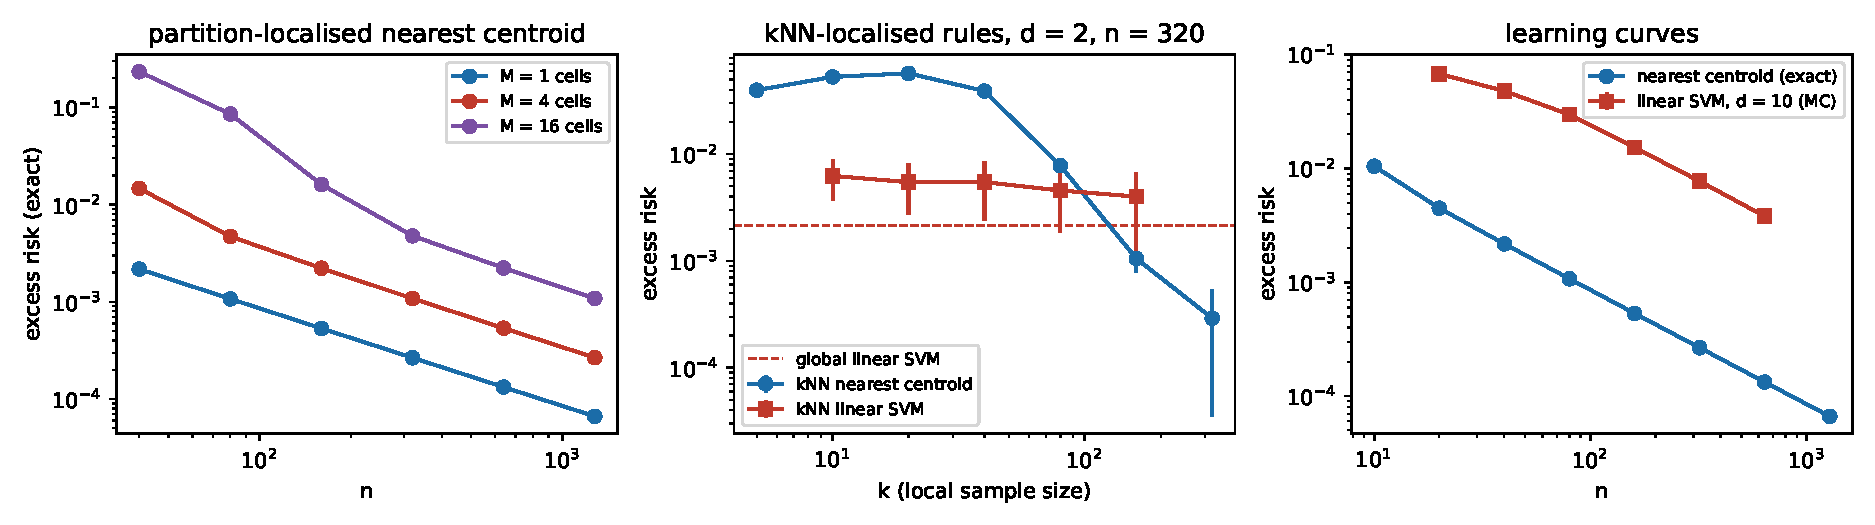
\includegraphics[width=\linewidth]{../figures/fig_exact.pdf}
\caption{Left: exact excess risk of the partition-localised nearest-centroid rule against $n$ for $M=1,4,16$ label-independent cells (Corollary~\ref{cor:exact}). Middle: kNN-localised rules in $d=2$ (simulations D1, D2 of Appendix~\ref{app:sim}); the dashed line is the global linear SVM. Right: learning curves of the nearest-centroid threshold (exact) and of the linear SVM in $d=10$ (Monte Carlo, D3).}
\label{fig:exact}
\end{figure}

\paragraph{Rules not covered by the proposition.} Appendix~\ref{app:sim} and Figure~\ref{fig:exact} report simulations in the same model for the rules the proposition does not cover (computationally verified, not proved): the kNN-localised nearest-centroid rule in $d=2$ is at worst about twice as bad as the global one (at $k=\ExKnnCWorstK$: $\ExKnnCWorst$ against $\ExKnnCThreeTwoZero$), the kNN-localised linear SVM in $d=2$ is within simulation error of the global linear SVM for $k\ge20$, the learning curve of the global linear SVM in $d=10$ is \ExSvmCurveMonotone{} (the monotonicity that Proposition~\ref{prop:thin} needs), and accordingly the partition-localised linear SVM with label-independent cells grows with $M$ ($\ExSvmPartOne$, $\ExSvmPartTwo$, $\ExSvmPartFour$, $\ExSvmPartEight$ for $M=1,2,4,8$).

\section{Experimental protocol and predefined criterion}\label{sec:protocol}

\paragraph{Data sets.} Six binary tasks (Table~\ref{tab:datasets}), grouped into three named regimes fixed before running: \emph{real} (wine, class 0 against the rest; breast cancer; digits, even against odd, a task with several modes per class), \emph{linear} (the Gaussian location model of Section~\ref{sec:theory} in $d=\DGauss$, $\delta=\ExDelta$, Bayes error $\ExBayes$, so that the linear reference contains the Bayes rule), and \emph{multiscale}, designed to favour local adaptation: two-scale moons (100 points of the standard moons and 300 points of a copy shrunk by 4 and displaced, so that scale and density both vary) and a two-scale checkerboard (100 points on $2\times2$ cells of side 1 and 300 points on $4\times4$ cells of side $\tfrac12$). Breast cancer and digits are subsampled (stratified) to 300 and 400 points and digits are reduced to 16 principal components fitted on the training fold; this subsampling is part of the compute budget and is stated as such.

\begin{table}[t]
\centering\small
\begin{tabular}{llrrrrr}
\toprule
data set & regime & $n$ & $d$ & $n_{\mathrm{train}}$ (main) & $n_{\mathrm{train}}$ (sub\SubFrac) & positives\\
\midrule
wine & real & 178 & 13 & 142 & 40 & 33\% \\
breast cancer & real & 300 & 30 & 240 & 60 & 63\% \\
digits (parity) & real & 400 & 64 & 320 & 80 & 50\% \\
Gaussian, linear & linear & 400 & 10 & 320 & 80 & 48\% \\
two-scale moons & multiscale & 400 & 2 & 320 & 80 & 50\% \\
two-scale checkerboard & multiscale & 400 & 2 & 320 & 80 & 52\% \\
\\
\bottomrule
\end{tabular}
\caption{Data sets. $d$ is the dimension after preprocessing (digits: 16 principal components). All inputs are standardised on the training fold.}
\label{tab:datasets}
\end{table}

\paragraph{Resampling and tuning.} Main condition: \NMainRepeats{} repetitions of stratified 5-fold cross-validation (\NMainFolds{} outer folds). Two robustness conditions with \NRobFolds{} outer folds each, on a partition different from the main one: \emph{noise\NoiseRate}, in which each \emph{training} label of a fold is flipped independently with probability \NoiseProb{} (test labels clean), and \emph{sub\SubFrac}, in which only \SubFrac\% of the training fold (stratified, at least 40 points) is used. Every family is tuned on the training fold by an inner stratified \InnerFolds-fold cross-validation with accuracy as the score. Grids: linear SVM $C\in\{\CLin\}$; RBF-SVM $C\in\{\CRbf\}$, $\gamma\in\{\GammaMults\}\times\gamma_{\mathrm{med}}$ with $\gamma_{\mathrm{med}}$ the inverse median squared distance; kNN-SVM $k\in\{\KnnKs,\text{all}\}$ with $C=\KnnC$ fixed, the inner validation sets being subsampled to at most \KnnValCap{} points to bound the number of per-point fits; cell-SVM $M\in\{\CellMs\}$, $C\in\{\CellCs\}$; VB-RBF-SVM the RBF grid times $\beta\in\{\VbBetas\}$ with $\kappa=\VbKbw$; LLSVM $M\in\{\LlsvmMs\}$, $C\in\{\LlsvmCs\}$ (values of $M$ exceeding the number of points of an inner training fold are dropped in that fold, which only happens under sub\SubFrac). Ties are broken towards the global member (Remark~\ref{rem:nesting}). These grids are those of v0.2: in the first run (v0.1) the grids were $C\le10$, $\gamma\le10\gamma_{\mathrm{med}}$, $M\le8$ and $k\ge20$, and the inner cross-validation selected an edge value in most folds of the data sets that decide the result (the RBF reference chose $\gamma=10\gamma_{\mathrm{med}}$ and $C=10$ in all 20 multiscale folds; cell-SVM and LLSVM chose $M=8$ in 14--16 of them and in all digits folds; kNN-SVM chose $k=20$ in 15 of them), so the grids were widened at those ends, the widening was recorded before running, in the file \path{PREREGISTRO_SVMF001.md} kept with the sources, and the fraction of folds that select an edge value is now reported (Table~\ref{tab:edge}).

\paragraph{Reference and paired comparison.} The \emph{best global reference} in an outer fold is whichever of the linear and RBF-SVM has the higher inner-cross-validation score in that fold, the RBF-SVM only if its score is strictly higher (ties go to the linear SVM); its test accuracy is the reference value, so the choice uses no test data. For each family and data set we record the paired difference (family minus reference) in each outer fold and a percentile bootstrap 95\% interval of the mean difference over folds ($B=2000$)~\citep{efron1993}; an interval whose endpoint is exactly zero counts as including zero. Outer folds of a cross-validation are not independent, so these intervals are descriptive rather than exact~\citep{dietterich1998,nadeau2003}, and with \NDatasets{} data sets no formal multi-data-set test is attempted~\citep{demsar2006}; with \NMainFolds{} folds they are also wide, which works against detecting small effects in either direction. With \NCellsMain{} intervals at the 95\% level in the main condition (\NCellsAll{} over the three conditions), about \ExpectedFalseMain{} (\ExpectedFalseAll) are expected to exclude zero by chance alone under no true difference; the majority clause of the criterion below is meant to absorb this, the single-data-set regime clause is not.

\paragraph{Predefined criterion of added value.} A family has \emph{added value} if (A) its mean paired improvement over the best global reference is positive with a bootstrap interval excluding zero on a majority of the \NDatasets{} data sets in the main condition; or, failing that, (B) there is a named regime on every data set of which (A) holds, and no data set outside the regime shows an interval entirely below zero. Robustness is reported separately as the accuracy under the two conditions and the paired differences there. The criterion, the regimes, the families, the seed and the v0.1 grids were fixed in the code before the first run, but not in a dated record independent of the code, so that statement rests on the authors' word; the v0.2 widening of the grids and everything else that was to be done with the new results was written down and dated before the re-run. One sensitivity check added after seeing the v0.1 results (the oracle reference of Section~\ref{sec:results}) is labelled as post hoc.

\section{Results}\label{sec:results}

\subsection{Main condition}

Table~\ref{tab:main} gives the mean accuracies of the two references and of the selected reference together with the paired differences of the four families against the selected reference; Figure~\ref{fig:paired} shows all three conditions, and \path{results/tables.md} has the accuracies of every method. Of the \NCellsMain{} data-set/family cells, \NNegCellsMain{} have intervals entirely below zero, \NPosCellsMain{} entirely above (\PosCellsMain), and the rest include zero.

\begin{table}[t]
\centering\footnotesize
\setlength{\tabcolsep}{2.5pt}
\begin{tabular}{lrrrrrrr}
\toprule
& \multicolumn{3}{c}{accuracy (\%)} & \multicolumn{4}{c}{paired difference vs.\ selected reference (pp), mean and 95\% interval}\\
\cmidrule(lr){2-4}\cmidrule(lr){5-8}
data set & linear & RBF & selected & kNN-SVM & cell-SVM & VB-RBF-SVM & LLSVM\\
\midrule
wine & 99.2 & 99.7 & 99.7 & -0.28 & \textbf{-1.42} & +0.00 & -0.57 \\
&  &  &  & [-1.11,\,+0.56] & [-2.83,\,-0.01] & [+0.00,\,+0.00] & [-1.67,\,+0.54] \\
\addlinespace[1.5pt]
breast cancer & 96.0 & 96.0 & 96.5 & -1.33 & -0.33 & -0.50 & -0.33 \\
&  &  &  & [-3.34,\,+0.67] & [-1.33,\,+0.50] & [-1.33,\,+0.00] & [-1.50,\,+0.67] \\
\addlinespace[1.5pt]
digits & 85.2 & 97.5 & 97.5 & +0.75 & \textbf{-2.00} & +0.13 & \textbf{-1.13} \\
&  &  &  & [-0.50,\,+2.00] & [-3.50,\,-0.37] & [-0.37,\,+0.75] & [-2.25,\,-0.13] \\
\addlinespace[1.5pt]
Gaussian & 93.9 & 93.5 & 93.3 & \textbf{-2.62} & -0.25 & \textbf{+0.37} & -0.12 \\
&  &  &  & [-3.88,\,-1.62] & [-1.12,\,+0.50] & [+0.12,\,+0.75] & [-0.87,\,+0.63] \\
\addlinespace[1.5pt]
moons & 84.5 & 97.0 & 97.0 & -0.37 & \textbf{-3.75} & +0.12 & \textbf{-7.38} \\
&  &  &  & [-1.63,\,+1.00] & [-5.88,\,-1.25] & [-1.25,\,+1.37] & [-9.13,\,-5.75] \\
\addlinespace[1.5pt]
checkerboard & 50.8 & 89.4 & 89.4 & \textbf{-3.50} & \textbf{-7.63} & +0.50 & \textbf{-4.88} \\
&  &  &  & [-6.38,\,-0.50] & [-11.38,\,-3.25] & [-0.50,\,+2.12] & [-7.63,\,-1.87]
\\
\bottomrule
\end{tabular}
\caption{Main condition, \NMainFolds{} outer folds. ``Selected'' is the best global reference chosen by inner cross-validation in each fold; it can be below both references' means because it is a per-fold choice. Differences are family minus selected reference, in percentage points, with the percentile bootstrap 95\% interval beneath; bold marks an interval that excludes zero.}
\label{tab:main}
\end{table}

\begin{figure}[t]
\centering
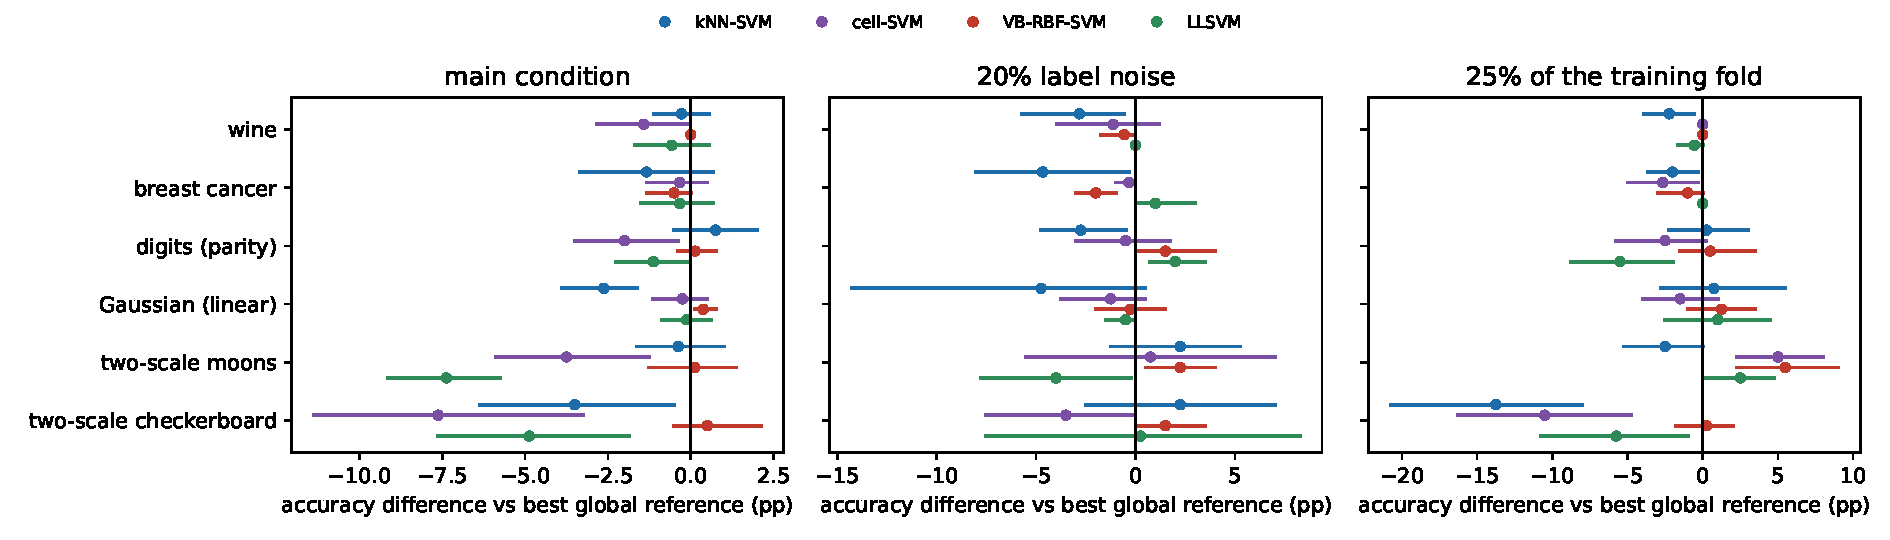
\includegraphics[width=\linewidth]{../figures/fig_paired.pdf}
\caption{Paired accuracy differences against the selected best global reference (percentage points) with bootstrap 95\% intervals, for the main condition and the two robustness conditions.}
\label{fig:paired}
\end{figure}

\paragraph{Local linear families.} The three local \emph{linear} families (kNN-SVM, cell-SVM, LLSVM) are never significantly better and are significantly worse wherever the RBF-SVM is much better than the linear SVM: digits (cell-SVM $\DiffMainDigCell$, LLSVM $\DiffMainDigLlsvm$), two-scale moons ($\DiffMainMoonsKnn$, $\DiffMainMoonsCell$, $\DiffMainMoonsLlsvm$) and the checkerboard ($\DiffMainCheckKnn$, $\DiffMainCheckCell$, $\DiffMainCheckLlsvm$). With $\NTrainMainMoons$ training points, piecewise-linear boundaries built from local linear SVMs do not reach the RBF-SVM on curved boundaries at two scales (Figure~\ref{fig:regions} in Appendix~\ref{app:tables} shows the fitted regions). Table~\ref{tab:edge} says how far this is a property of the families rather than of the grids: the counts of folds in which the inner cross-validation selected an edge value of the widened grids are given per data set and hyper-parameter, and the text of Section~\ref{sec:claims} states which conclusions remain grid-limited.

\paragraph{The variable-bandwidth family.} VB-RBF-SVM, which contains the RBF-SVM, is statistically indistinguishable from the selected reference on the two multiscale sets for which it was designed ($\DiffMainMoonsVb$ [$\DiffLoMainMoonsVb$, $\DiffHiMainMoonsVb$] and $\DiffMainCheckVb$ [$\DiffLoMainCheckVb$, $\DiffHiMainCheckVb$]) and on the three real data sets, and shows $\DiffMainGaussVb$ [$\DiffLoMainGaussVb$, $\DiffHiMainGaussVb$] on the Gaussian linear data set, where Section~\ref{sec:theory} says that local adaptation cannot reduce the excess risk. Table~\ref{tab:main} explains the Gaussian cell: the linear SVM ($\AccMainGaussLin$) and the VB-RBF-SVM ($\AccMainGaussVb$) have about the same mean accuracy and both exceed the \emph{selected} reference ($\AccMainGaussBest$), because the inner cross-validation picked the RBF-SVM in \PickRbfMainGauss\% of the folds although the linear SVM was better on the test folds; this is the selection noise of Remark~\ref{rem:nesting}. Two checks confirm it. Against the family's own fixed global member, the RBF-SVM with the same grid, the difference is $\NestMainGaussVb$ [$\NestLoMainGaussVb$, $\NestHiMainGaussVb$], and across the \NCellsMain{} main-condition cells no family is significantly above its own global member (Table~\ref{tab:nested}). Against the post-hoc \emph{oracle} reference, the better of the two global references on each test fold (an optimistic reference, since it uses test data; defined after the v0.1 results were seen), the Gaussian cell is $\PostMainGaussVb$ [$\PostLoMainGaussVb$, $\PostHiMainGaussVb$] and no interval is above zero anywhere (\PostNPosAll{} of \PostNCellsAll{} cells across all conditions). Finally, the inner cross-validation did select genuinely local configurations: a $\beta>0$ in \LocalFracMainGaussVb\% of the Gaussian folds and in \LocalFracMainMoonsVb\% and \LocalFracMainCheckVb\% of the multiscale folds, and $M>1$ or $k\ne$ all in most folds of the data sets where the local linear families then lose (\path{results/tables.md}), so the families were not simply collapsed onto their global members.

\begin{table}[t]
\centering\small
\setlength{\tabcolsep}{4pt}
\begin{tabular}{lrrrrrrr}
\toprule
method: hyper-parameter & wine & breast c. & digits & Gaussian & moons & checkerb. & all\\
\midrule
linear SVM: $C$ & 0/0 & 0/1 & 0/2 & 0/1 & 0/3 & 7/1 & 7/8 \\
RBF-SVM: $\gamma$ & 2/0 & 5/0 & 0/0 & 8/0 & 0/0 & 0/0 & 15/0 \\
RBF-SVM: $C$ & 0/0 & 0/0 & 0/0 & 0/0 & 0/1 & 0/5 & 0/6 \\
kNN-SVM: $k$ & 1/-- & 2/-- & 8/-- & 0/-- & 10/-- & 10/-- & 31/-- \\
cell-SVM: $M$ & --/1 & --/0 & --/6 & --/0 & --/4 & --/7 & --/18 \\
cell-SVM: $C$ & 7/0 & 3/0 & 3/0 & 8/2 & 0/10 & 0/10 & 21/22 \\
VB-RBF-SVM: $\gamma$ & 2/0 & 4/0 & 0/0 & 7/0 & 0/6 & 0/0 & 13/6 \\
VB-RBF-SVM: $C$ & 0/0 & 0/0 & 0/0 & 0/0 & 0/0 & 0/4 & 0/4 \\
VB-RBF-SVM: $\beta$ & --/0 & --/0 & --/4 & --/2 & --/2 & --/3 & --/11 \\
LLSVM: $M$ & --/0 & --/1 & --/7 & --/1 & --/9 & --/10 & --/28 \\
LLSVM: $C$ & 0/0 & 0/2 & 0/10 & 4/1 & 0/9 & 0/10 & 4/32
\\
\bottomrule
\end{tabular}
\caption{Grid saturation in the main condition: number of outer folds (of \EdgeMainFoldsPerSet{} per data set, \EdgeMainAllRbfGammaN{} in all) in which the inner cross-validation selected the lowest/highest value of the widened grid (lower/upper, ``--'' when that edge is the family's global member and is not a saturation: $k=$ all, $M=1$, $\beta=0$). For $M$ the top of the grid available in the fold is used.}
\label{tab:edge}
\end{table}

\subsection{Robustness: label noise and subsampling}

Table~\ref{tab:robust} gives the accuracies averaged over data sets and their drops from the main condition; the per-data-set paired differences are in Figure~\ref{fig:paired} and \path{results/tables.md}. Under label noise the average accuracy of the selected reference falls by \DropNoiseBest{} points, and under subsampling by \DropSubBest{}; the local families fall by \DropNoiseKnn, \DropNoiseCell, \DropNoiseVb{} and \DropNoiseLlsvm{} points under noise and by \DropSubKnn, \DropSubCell, \DropSubVb{} and \DropSubLlsvm{} under subsampling (kNN-SVM, cell-SVM, VB-RBF-SVM, LLSVM). These drops are not comparable across families, because the three local linear families start from much lower accuracies on the curved data sets, and they also mix the effect of the condition with that of a different partition into folds; the paired comparison within each condition is the relevant one. There, no family is significantly above the reference under either condition (the largest positive differences are those of VB-RBF-SVM on the subsampled multiscale sets, $\DiffSubMoonsVb$ [$\DiffLoSubMoonsVb$, $\DiffHiSubMoonsVb$] and $\DiffSubCheckVb$ [$\DiffLoSubCheckVb$, $\DiffHiSubCheckVb$]; both include zero and are recorded as a hypothesis for a larger run, not as a result). The kNN-SVM, whose local fits see few and, under noise, mislabelled points, is significantly below the reference on \NNegNoiseKnn{} of \NDatasets{} data sets under noise and \NNegSubKnn{} under subsampling, against \NNegMainKnn{} in the main condition; VB-RBF-SVM is below on \NNegNoiseVb{} under noise and \NNegSubVb{} under subsampling. We therefore find no evidence of superior robustness for any family---which, with \NRobFolds{} folds and intervals several points wide, is not evidence of its absence---and a widening disadvantage for the neighbourhood-based family under both stresses, in line with the variance mechanism of Section~\ref{sec:theory}.

\begin{table}[t]
\centering\small
\begin{tabular}{lrrrrr}
\toprule
& main & \multicolumn{2}{c}{noise\NoiseRate} & \multicolumn{2}{c}{sub\SubFrac}\\
\cmidrule(lr){3-4}\cmidrule(lr){5-6}
method & acc. & acc. & drop & acc. & drop\\
\midrule
linear SVM & 84.9 & 83.0 & 1.9 & 82.5 & 2.4 \\
RBF-SVM & 95.5 & 88.4 & 7.1 & 89.3 & 6.2 \\
best global (inner CV) & 95.6 & 88.5 & 7.1 & 89.2 & 6.4 \\
kNN-SVM & 94.3 & 86.7 & 7.6 & 85.9 & 8.4 \\
cell-SVM & 93.0 & 87.5 & 5.5 & 87.2 & 5.8 \\
VB-RBF-SVM & 95.7 & 88.9 & 6.8 & 90.3 & 5.4 \\
LLSVM & 93.2 & 88.3 & 4.9 & 87.8 & 5.4
\\
\bottomrule
\end{tabular}
\caption{Accuracy (\%) averaged over the \NDatasets{} data sets in each condition, and drop from the main condition (percentage points). The robustness conditions use \NRobFolds{} outer folds on a partition different from the main one, so a drop mixes the effect of the condition with that of the partition.}
\label{tab:robust}
\end{table}

\subsection{Verdict under the predefined criterion}

Table~\ref{tab:criterion} applies the criterion of Section~\ref{sec:protocol} literally. No family meets the majority clause (A). The regime clause (B) is met, by the letter, by \NFamiliesAddedValue{} family--regime pair(s): \CritVbRegimes{} for VB-RBF-SVM, \CritKnnRegimes{} for kNN-SVM, \CritCellRegimes{} for cell-SVM, \CritLlsvmRegimes{} for LLSVM. Where the clause is met by the single-data-set \emph{linear} regime, we report it as the rule requires and say why it is not added value in the sense intended: the regime is the one in which Section~\ref{sec:theory} shows that no reduction of excess risk is available, the gain is against the selected reference and vanishes against the family's own global member and against the oracle reference, a one-data-set regime is too weak a base for a named-regime claim, and a single interval excluding zero among \NCellsMain{} is what chance alone would produce. The flaw is in our criterion, which should have required at least two data sets per regime; we record it rather than repair it after the fact. In the multiscale regime, for which the variable-bandwidth family was designed, the outcome is a tie with the RBF-SVM.

\begin{table}[t]
\centering\small
\begin{tabular}{lccclc}
\toprule
family & CI $>0$ & CI $<0$ & majority (A) & named regime (B) & added value\\
\midrule
kNN-SVM & 0/6 & 2/6 & not met & none & no \\
cell-SVM & 0/6 & 3/6 & not met & none & no \\
VB-RBF-SVM & 1/6 & 0/6 & not met & linear & yes (by the letter; see text) \\
LLSVM & 0/6 & 3/6 & not met & none & no \\
\\
\bottomrule
\end{tabular}
\caption{The predefined criterion applied to the main condition (\NDatasets{} data sets).}
\label{tab:criterion}
\end{table}

\section{What can be claimed}\label{sec:claims}

\begin{table}[!htbp]
\centering\small
\begin{tabular}{p{0.72\linewidth}p{0.20\linewidth}}
\toprule
claim & status\\
\midrule
If the reference class contains a Bayes rule, localisation can act only on the estimation term (Lemma~\ref{lem:approx}); $K_a$ is a positive-definite kernel that nests the RBF kernel (Lemma~\ref{lem:pd}) & proved here\\
Partition-localised rule with label-independent cells: risk is the learning curve averaged at binomially thinned sizes; not below the global rule if the curve is non-increasing, strictly above if $M\ge2$ and the curve decreases at the last step (Prop.~\ref{prop:thin}) & proved here\\
Nearest-centroid threshold in the Gaussian model: closed-form conditional risk, learning curve strictly decreasing for $n\ge1$ (Prop.~\ref{prop:exact}); partition-localisation with 4 cells at $n=\ExPartN$ multiplies the excess risk by $\ExPartRatioFour$ (Cor.~\ref{cor:exact}); Monte Carlo agrees to within one standard error & proved; exact numbers; verified\\
The linear SVM's learning curve is decreasing in the Gaussian model, $d=10$, and partition-localised SVM risk grows with $M$ (D3, D4); kNN-localised rules there do not improve on the global rule (D1, D2) & verified, not proved\\
No family meets the majority criterion of added value on \NDatasets{} data sets; the \NPosCellsMain{} interval(s) above zero are against the selected reference and are compatible with chance, and no family is above its own global member & measured\\
Local linear families are significantly worse than the reference on the curved multiscale sets and on digits, with the widened grids of Section~\ref{sec:protocol}; saturation that remains at an edge is listed in Table~\ref{tab:edge} & measured, grid-limited where Table~\ref{tab:edge} says so\\
VB-RBF-SVM ties the RBF-SVM on the multiscale sets & measured\\
No family is significantly above the reference under label noise or subsampling (no evidence of superior robustness); kNN-SVM is significantly below it on \NNegNoiseKnn{} and \NNegSubKnn{} of \NDatasets{} data sets & measured\\
General superiority of any family in accuracy or robustness; behaviour of the original variants, of larger samples, or of other kernels & not claimed / not addressed\\
\bottomrule
\end{tabular}
\caption{Claims and their status. ``Verified'' and ``measured'' mean produced by the scripts of Appendix~\ref{app:repro} with the fixed seed; neither is a proof.}
\label{tab:claims}
\end{table}

\paragraph{Limitations.} The families are reconstructions chosen for transparency, not the strongest versions in the literature: the local SVMs are linear with a fixed $C$, the cell and anchor partitions come from a single $k$-means run, the kNN-SVM's inner validation is subsampled, and the variable-bandwidth exponent takes three values. The data sets are small by design (a total budget of about \MetaSecondsTotal{} CPU-seconds), so the comparison speaks to the regime of a few hundred training points, where the variance mechanism of Section~\ref{sec:theory} is strongest and local methods are at a disadvantage; with much larger samples the balance may differ, and nothing here says otherwise. The hyper-parameter grids are finite, and where Table~\ref{tab:edge} shows selections at an edge the corresponding comparison is between methods limited by their grids. The bootstrap intervals treat the outer folds as exchangeable, which they are not, and no correction for the \NCellsMain{} simultaneous intervals is applied beyond the majority clause. Proposition~\ref{prop:thin} covers partitions independent of the labels; data-dependent partitions and neighbourhoods are only illustrated. The criterion's regime clause admitted a single-data-set regime, a design flaw reported above. The predefinition of the v0.1 protocol is not independently verifiable (Section~\ref{sec:protocol}).

\paragraph{Next steps for the research line.} (a) A lower bound for neighbourhood-based localisation: for the kNN-localised linear rule in the Gaussian model, bound the conditional excess risk at a query by the local sample size, which would extend Proposition~\ref{prop:thin} to the kNN-SVM. (b) Re-run the comparison at $n$ in the thousands with the same criterion (repaired to require two data sets per regime) to see whether the multiscale tie turns into a gain for the variable-bandwidth family. (c) Compare the variable-bandwidth kernel with the simpler alternative of a global RBF-SVM on density-normalised inputs, which may capture the same effect without the dimension-dependent prefactor of Lemma~\ref{lem:pd}. (d) If the original variants of the line are recovered, insert them into this protocol unchanged.

\clearpage
\appendix
\section{Reproducibility}\label{app:repro}
{\sloppy The directory contains \path{experiments/families.py} (the six families in about 300 lines), \path{experiments/run_comparison.py} (protocol, criterion, bootstrap, grid-saturation counts, \path{results/results.json}, \path{results/tables.md}, Figure~\ref{fig:paired}), \path{experiments/exact_example.py} (Section~\ref{sec:theory}: exact sums, Monte Carlo, D1--D4, \path{results/exact_example.json}, Figure~\ref{fig:exact}), \path{experiments/posthoc_oracle.py} (oracle and own-member comparisons, from \path{results.json} only), \path{experiments/make_region_figure.py} (Figure~\ref{fig:regions}) and \path{experiments/make_numbers.py}, which converts the JSON results into the macros and table bodies used by this document, so that no number in the text is typed. Seed \MetaSeed; Python \MetaPython, NumPy \MetaNumpy, SciPy \MetaScipy, scikit-learn \MetaSklearn~\citep{pedregosa2011}; single-threaded BLAS; \MetaSecondsMain{} seconds for the comparison and \MetaSecondsExact{} seconds for the exact example on a shared four-core machine. \path{run_comparison.py} with \texttt{--fast} runs a reduced smoke test; the v0.1 results are kept in \path{results/v01/}. Implementation details (preprocessing, inner-fold seeds, shared $k$-means partitions, reuse of the RBF inner scores for $\beta=0$) are in the README. One detail matters for Lemma~\ref{lem:pd}: the implementation computes $r_\kappa$ excluding the point itself for training points and not for queries, so the bandwidth map is not a single function of $x$ at the training points and $K_a(z,x_i)\not\to1$ as $z\to x_i$; the training Gram matrix is $K_a$ for the map restricted to the training set, so its positive semidefiniteness and all reported numbers are unaffected.\par}

\section{Simulations for rules not covered by Proposition~\ref{prop:thin}}\label{app:sim}
The middle and right panels of Figure~\ref{fig:exact} report simulations in the model of Proposition~\ref{prop:exact} (computationally verified, not proved); the full tables, with standard errors, are in \path{results/exact_example.md}. D1 uses \ExDoneReps{} training samples and the exact conditional risk averaged over \ExDoneTest{} test points; D2 \ExDtwoReps{} samples and \ExDtwoTest{} test points with $C=1$ (its ``global'' value is the exact risk of the fitted hyperplane and its kNN values the exact conditional risk averaged over the test points, two different estimators of the same quantity); D3 \ExDthreeReps{} samples per $n$; D4 \ExDfourReps{} samples with cells drawn independently of the data. (D1) The kNN-localised nearest-centroid rule in $d=2$ (second coordinate pure noise), $n=\ExPartN$: the risk is worst at $k=\ExKnnCWorstK$ ($\ExKnnCWorst$, against $\ExKnnCThreeTwoZero$ for $k=n$), because the local class means are truncated by the neighbourhood (bias) and computed from few points (variance); for small $k$ the neighbourhoods are mostly pure and the rule degenerates to a $k$-NN vote~\citep{cover1967,stone1977}. (D2) The kNN-localised linear SVM in $d=2$ with $C=1$: $\ExKnnSOneZero$ at $k=10$ and $\ExKnnSOneSixZero$ at $k=160$ against $\ExKnnSAll\pm\ExKnnSSeAll$ for the global linear SVM; the differences at $k\ge20$ are about one simulation standard error, so in two dimensions the localised SVM neither helps nor clearly hurts here. (D3) The learning curve of the global linear SVM in $d=10$ is \ExSvmCurveMonotone{} between $n=20$ ($\ExSvmCurveTwoZero$) and $n=640$ ($\ExSvmCurveSixFourZero$). (D4) The partition-localised linear SVM with label-independent cells in $d=10$, $n=\ExPartN$, has risk $\ExSvmPartOne$, $\ExSvmPartTwo$, $\ExSvmPartFour$, $\ExSvmPartEight$ for $M=1,2,4,8$.


\section{Nested comparison and decision regions}\label{app:tables}
The mean accuracy of every method in every condition, the per-data-set paired differences of the two robustness conditions, the fraction of folds in which a local configuration was selected, and the grid-saturation counts of the robustness conditions are in \path{results/tables.md}; the post-hoc comparisons against the oracle reference are in \path{results/posthoc_oracle.md}. Table~\ref{tab:nested} and Figure~\ref{fig:regions} are kept here because the text relies on them.

\begin{table}[htbp]
\centering\footnotesize
\setlength{\tabcolsep}{4pt}
\begin{tabular}{lrrrr}
\toprule
& kNN-SVM & cell-SVM & VB-RBF-SVM & LLSVM\\
data set & vs.\ linear SVM & vs.\ linear SVM & vs.\ RBF-SVM & vs.\ linear SVM\\
\midrule
wine & +0.29 & -0.85 & +0.00 & +0.00 \\
& [-0.56,\,+1.15] & [-1.70,\,+0.00] & [+0.00,\,+0.00] & [+0.00,\,+0.00] \\
\addlinespace[1.5pt]
breast cancer & -0.83 & +0.17 & +0.00 & +0.17 \\
& [-2.33,\,+0.50] & [-0.33,\,+0.67] & [+0.00,\,+0.00] & [-1.00,\,+1.17] \\
\addlinespace[1.5pt]
digits (parity) & \textbf{+13.00} & \textbf{+10.25} & +0.13 & \textbf{+11.12} \\
& [+11.50,\,+14.50] & [+8.12,\,+12.25] & [-0.37,\,+0.75] & [+8.87,\,+13.12] \\
\addlinespace[1.5pt]
Gaussian (linear) & \textbf{-3.25} & -0.87 & +0.12 & -0.75 \\
& [-5.12,\,-1.63] & [-2.12,\,+0.25] & [-0.25,\,+0.50] & [-1.87,\,+0.25] \\
\addlinespace[1.5pt]
two-scale moons & \textbf{+12.12} & \textbf{+8.75} & +0.12 & \textbf{+5.12} \\
& [+10.50,\,+13.62] & [+6.00,\,+11.50] & [-1.25,\,+1.38] & [+3.75,\,+6.38] \\
\addlinespace[1.5pt]
two-scale checkerboard & \textbf{+35.12} & \textbf{+31.00} & +0.50 & \textbf{+33.75} \\
& [+32.25,\,+37.88] & [+27.38,\,+34.38] & [-0.50,\,+2.12] & [+31.00,\,+36.38]
\\
\bottomrule
\end{tabular}
\caption{Nested comparison, main condition: each family against its own fixed global reference (the tuned linear SVM for the three local linear families, the tuned RBF-SVM for VB-RBF-SVM), percentage points with 95\% intervals, bold when the interval excludes zero. For kNN-SVM the member actually contained in its grid is the linear SVM with $C=\KnnC$ fixed, so its column is an approximation of the nested comparison. \NestNPosMain{} intervals are above zero and \NestNNegMain{} below.}
\label{tab:nested}
\end{table}

\begin{figure}[htbp]
\centering
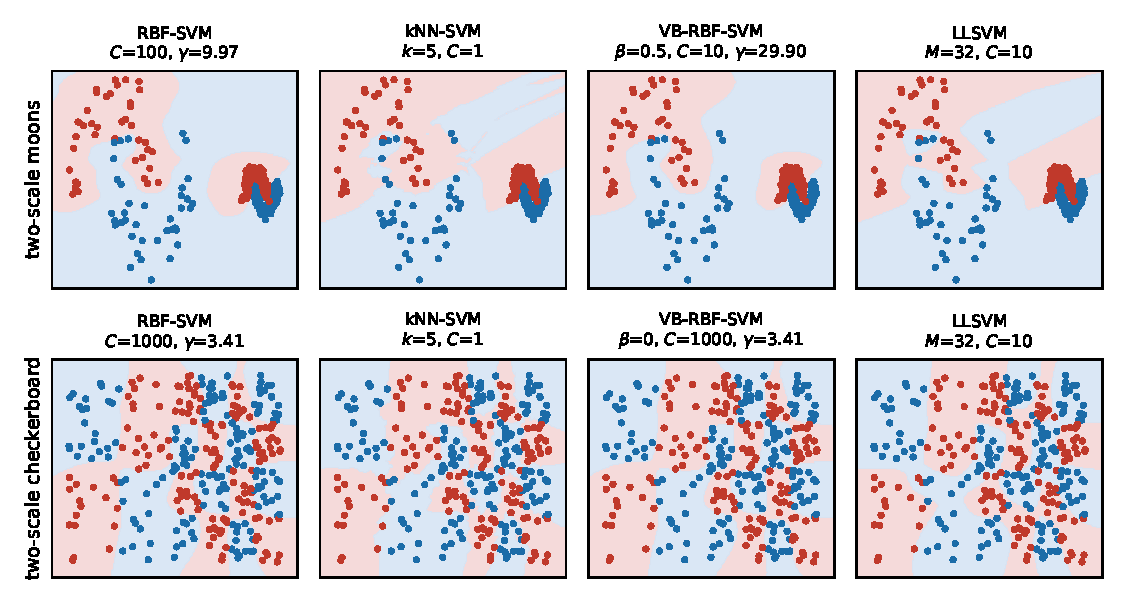
\includegraphics[width=\linewidth]{../figures/fig_regions.pdf}
\caption{Decision regions on the first outer training fold of the two multiscale data sets, for the configurations selected by inner cross-validation in that fold (given in the panel titles).}
\label{fig:regions}
\end{figure}

\bibliographystyle{plainnat}
\bibliography{refs}
\end{document}
